\documentclass{myBeamer}


\DeclareMathOperator{\Cov}{Cov}
\DeclareMathOperator{\Var}{Var}
\DeclareMathOperator{\E}{\mathbb{E}}
\DeclareMathOperator{\Proba}{\mathbb{P}}

\newcommand{\Covb}[2]{\ensuremath{\Cov\!\left[#1,#2\right]}}
\newcommand{\Eb}[1]{\ensuremath{\E\!\left[#1\right]}}
\newcommand{\Pb}[1]{\ensuremath{\Proba\!\left[#1\right]}}
\newcommand{\Varb}[1]{\ensuremath{\Var\!\left[#1\right]}}

% norm
%\newcommand{\norm}[1]{\| #1 \|}

\newcommand{\indep}{\rotatebox[origin=c]{90}{$\models$}}





\usepackage{mathptmx,amsmath,amssymb,graphicx,bibentry,bbm,babel,ragged2e,mdframed}

\makeatletter


\renewcommand{\addlogo}{
	\hfill	
	
\includegraphics[height=.4cm]{figures/iconOM.png}
	
\includegraphics[scale=1]{figures/openmole_dark.png}
}


\newcommand{\noun}[1]{\textsc{#1}}
\newcommand{\jitem}[1]{\item \begin{justify} #1 \end{justify} \vfill{}}
%\newcommand{\sframe}[2]{\frame{\frametitle{#1}\addlogo #2}}

\newenvironment{centercolumns}{\begin{columns}[c]}{\end{columns}}
%\newenvironment{jitem}{\begin{justify}\begin{itemize}}{\end{itemize}\end{justify}}

%\usetheme{Warsaw}
%\setbeamertemplate{footline}[text line]{}
%\setbeamersize{text margin left=15pt,text margin right=15pt}
%\setbeamertemplate{headline}{}
%\setbeamertemplate{footline}[frame number]
%\setbeamertemplate{navigation symbols}{}

\usetheme{Darmstadt}
\setbeamertemplate{headline}{}
\setbeamertemplate{navigation symbols}{}
\setbeamercolor{palette quaternary}{fg=primaryDarkOM, bg=primaryGreenOM}


%\setbeamercovered{transparent}
%\setbeamercolor{structure}{fg=purple!50!blue, bg=purple!50!blue}

\@ifundefined{showcaptionsetup}{}{%
 \PassOptionsToPackage{caption=false}{subfig}}
\usepackage{subfig}

\usepackage[utf8]{inputenc}
%\usepackage[T1]{fontenc}


\usepackage{tikz}

\usepackage{multirow}

\usepackage{mdframed}

%\usepackage[usenames,dvipsnames]{pstricks}
%\usepackage{auto-pst-pdf}


%\usepackage[dvipsnames]{xcolor}

\usepackage{threeparttable}


\usepackage{listings}
\lstset{language=Java} 

\makeatother


\usepackage{csquotes}
\usepackage{pifont}
%\newcommand{\cmark}{\textcolor{green}\ding{51}}
%\newcommand{\xmark}{\textcolor{red}\ding{55}}
\newcommand{\cmark}{\ding{51}}
\newcommand{\xmark}{\ding{55}}

\title[eXModelo feedback]{Fostering the use of methods for geosimulation models sensitivity analysis and validation}

\author{\tiny\noun{R. Reuillon}$^{1,2}$, \noun{M. Leclaire}$^{1,2}$, \noun{J. Raimbault}$^{3,1,2,\ast}$, \noun{H. Arduin}$^4$, \noun{P. Chapron}$^5$, \noun{G. Ch{\'e}rel}$^1$, \noun{E. Delay}$^6$, \noun{F. Lavall{\'e}e}$^7$, \noun{J. Passerat}$^8$, \noun{P. Peigne}$^9$, \noun{J. Perret}$^{1,5}$, \noun{S. Rey-Coyrehourcq}$^{10}$}

%Juste devrait être premier auteur non ? (il me semble que c'est lui qui a écrit le petit abstract)  
% comme c'est Romain et Mathieu qui ont créé exmodelo ca semble plus logique - too late anyway l'abstract est published.

\institute{\tiny
$^1$ UPS CNRS 3611 ISC-PIF\\
$^2$ UMR CNRS 8504 G{\'e}ographie-cit{\'e}s\\
$^3$ CASA, UCL\\
$^4$ UMR Inserm 1037 CRCT\\
$^5$ Univ. Paris-Est, LaSTIG STRUDEL, IGN, ENSG\\
$^6$ CIRAD UPR GREEN\\%, F-34398 Montpellier, France\\
$^7$ Irstea, LISC \\
$^8$ ConsenSys\\
$^9$ {\'E}cole 42\\
$^{10}$ UMR CNRS 6266 IDEES\medskip\\
$^{\ast}$ juste.raimbault@polytechnique.edu\medskip\\

\includegraphics[scale=2]{figures/openmole.png}
}

\date{\footnotesize ECTQG 2019\\
Exploration of geosimulation models\\
September 6th, 2019}

\begin{document}



\begin{frame}[plain]
	\titlepage
\end{frame}


%\textit{Validation of simulation models; Multi-modeling; Model calibration; Sensitivity analysis; Incremental modeling; Pedagogy of simulation models}


\sframe{Simulation in TQG}{

\begin{columns}

	\begin{column}{0.5\textwidth}
	\centering
	
	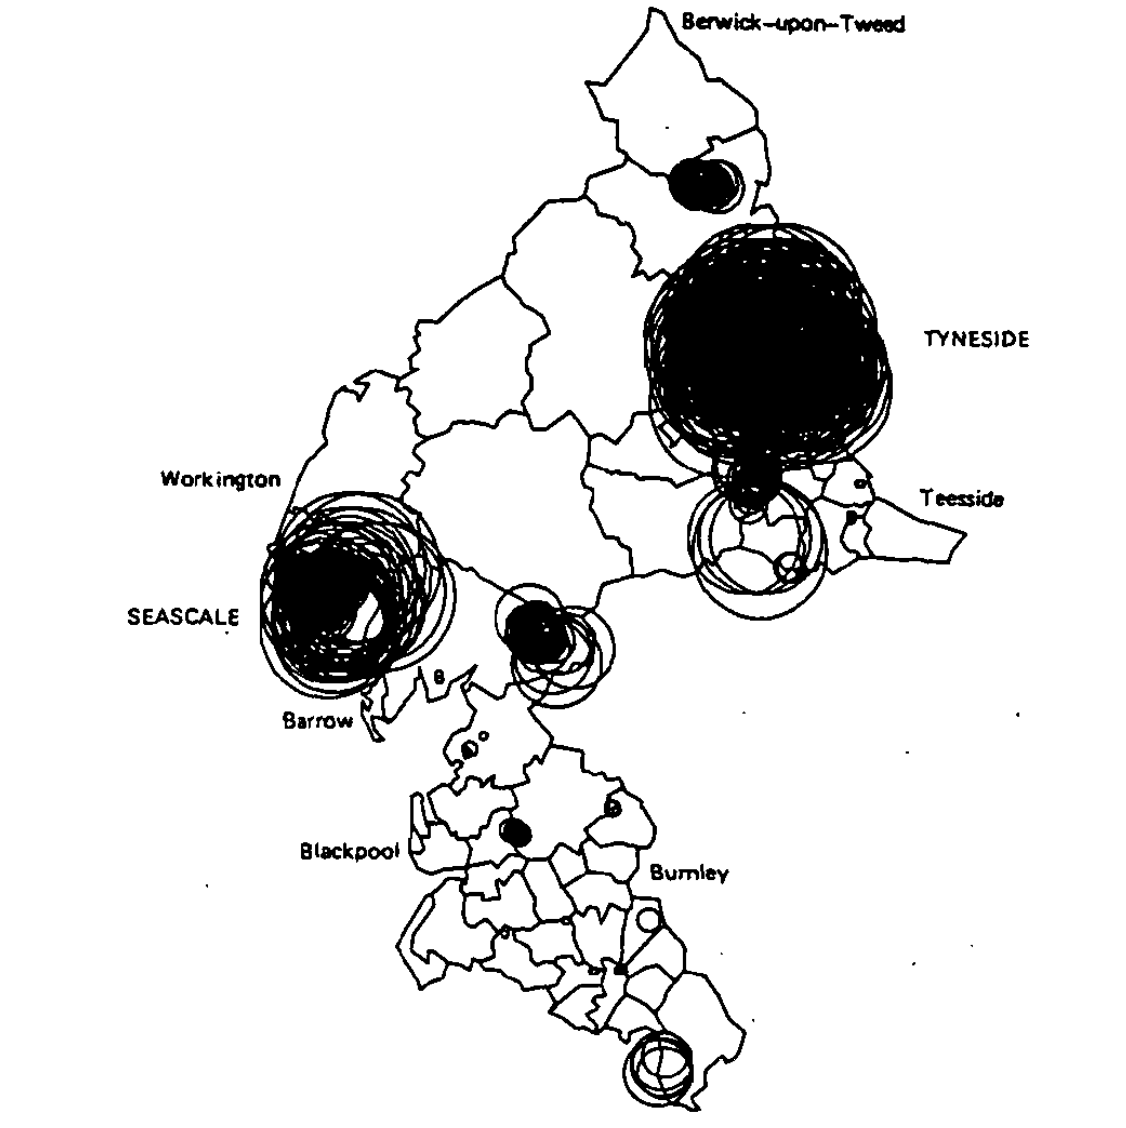
\includegraphics[width=0.6\textwidth]{figures/openshaw.png}
	
	\footnotesize
\textit{Geographical analysis machine \cite{openshaw1987mark}}
	
	\medskip
	\hrule
	\medskip
	
	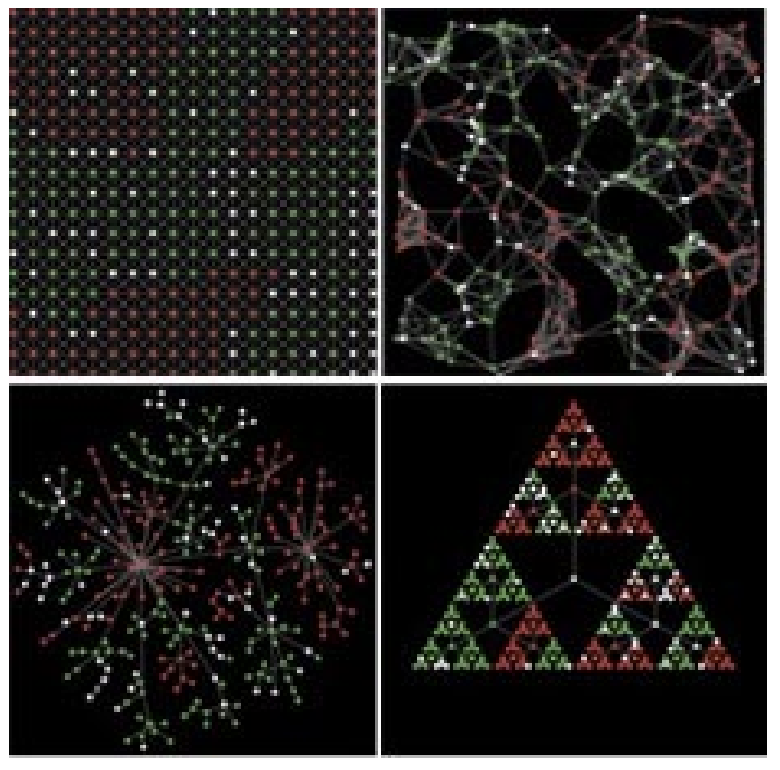
\includegraphics[width=0.55\textwidth,height=0.3\textheight]{figures/banos-schelling.png}
	
	\footnotesize
\textit{Schelling on networks \cite{banos2012network}}
	

	\end{column}
	\vrule{}
	\begin{column}{0.5\textwidth}
	\centering
	
	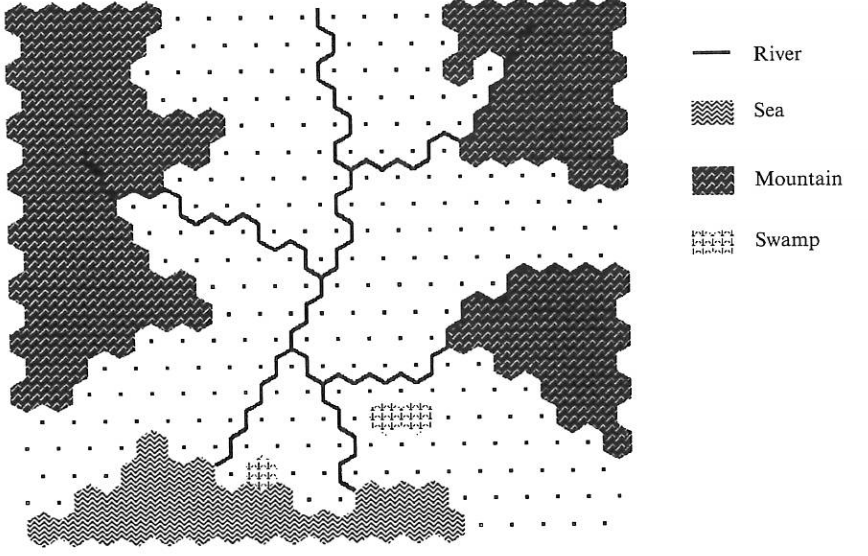
\includegraphics[width=0.7\textwidth]{figures/simpop1.png}
	
	\footnotesize
\textit{Simpop 1 model\cite{sanders1997simpop}}

	\medskip

	\hrule
	
	\medskip

	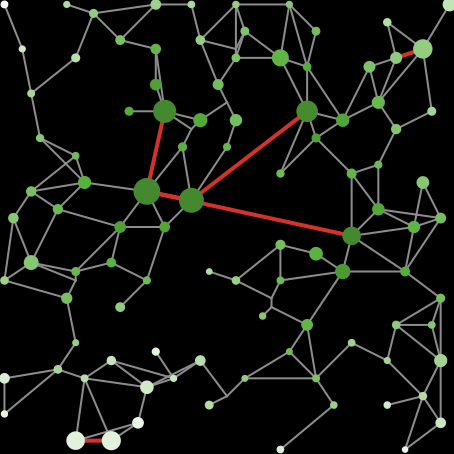
\includegraphics[width=0.6\textwidth]{figures/setup_synth_1_tick100.png}
	
	\footnotesize
	\textit{SimpopNet model \cite{schmitt2014modelisation}}
	
	\end{column}


\end{columns}

}


\sframe{Geographical systems and complexity}{

% pour laquelle la prépondérance de l'espace augmente la complexité des modèles

\textit{Necessity of simulation models in geography induced by complexities of these systems ?}

\bigskip

\begin{itemize}
	\item Ontological complexity \cite{pumain2003approche}
	\item Dynamical complexity: non-ergodicity and path-dependancy \cite{pumain2012urban}
	\item Complexity and co-evolution
	\item Complexity and emergence
\end{itemize}

}




\sframe{Exploration of geosimulation models}{

\justify

\textbf{Model exploration} is basically running a model \emph{a lot of times}, following a \emph{design of experiments}, to gain knowledge about \emph{model properties}.

\medskip

e.g. : sensitivity analysis 

\bigskip

Recent and significant increase in the development of methods to explore, calibrate and optimize (geo)simulation models.

\bigskip

$\rightarrow$ ease model validation !
%In recent years, there has been a significant increase in the development of methods to explore, validate, calibrate and optimize geosimulation models.

}


\sframe{Practice of model validation}{

Methods and tools remain underused  by simulation communities, despite an easier access to HPC facilities.

\bigskip

\begin{small}
e.g. mail of Bruce Edmonds (emblematic figure of social simulation) on the SIMSOC mailing list, on the 16\textsuperscript{th} of May 2019.

\begin{mdframed}
\begin{displayquote}
Dear Colleagues,

David Hales and I have been looking at \textbf{how to do massively parallel runs of NetLogo simulation models on the Cloud}. Something like (a) design your runs using NetLogo's BehaviorSpace (b) upload the model to the cloud (c) run it on the cloud (d) get the resulting table of results back.

We are wondering how many people would be interested in something like this.[...]


\end{displayquote}
\end{mdframed}
\end{small}
}


\sframe{OpenMOLE}{

%The OpenMOLE model exploration software~\citep{reuillon2013openmole} is one of the reliable approaches fully dedicated to promote these techniques.

% - promote OML + success stories

\justify

The \textbf{OpenMOLE} free and open source software provides (i) model embedding; (ii) transparent access to HPC; (iii) state-of-the-art model exploration methods.

\medskip

\begin{center}
    
\includegraphics[width=0.2\textwidth]{figures/iconOM.png}
    
\includegraphics[width=0.5\linewidth]{figures/openmole.png}
\end{center}

\medskip

\textbf{Success stories: } epidemiology \cite{arduin2018modelisation}, ecology 
\\\cite{lavallee2019stochastic}, planning \cite{brasebin2017apports},\\
urban science \cite{raimbault2018indirect}

}


\sframe{A researcher school on model exploration}{

%This presentation offers some feedback on the recent initiative of a researcher school in model validation, focused around models and practices linked to the OpenMOLE platform.

% - "not" an OpenMOlE school (although in practice it is)
% - between a formal summer school and workshop based formats (MAPS)

The \textbf{eXModelo school} to learn model validation methods

\medskip

\begin{center}
    
\includegraphics[width=0.9\textwidth]{figures/exmodelobanner.png}
\end{center}

\medskip

\begin{itemize}
    \item OpenMOLE as the learning tool, but reproducible with other tools and methods
    \item between a formal summer school and a workshop (student projects)
\end{itemize}


}


\sframe{Passionated researchers...}{

\centering

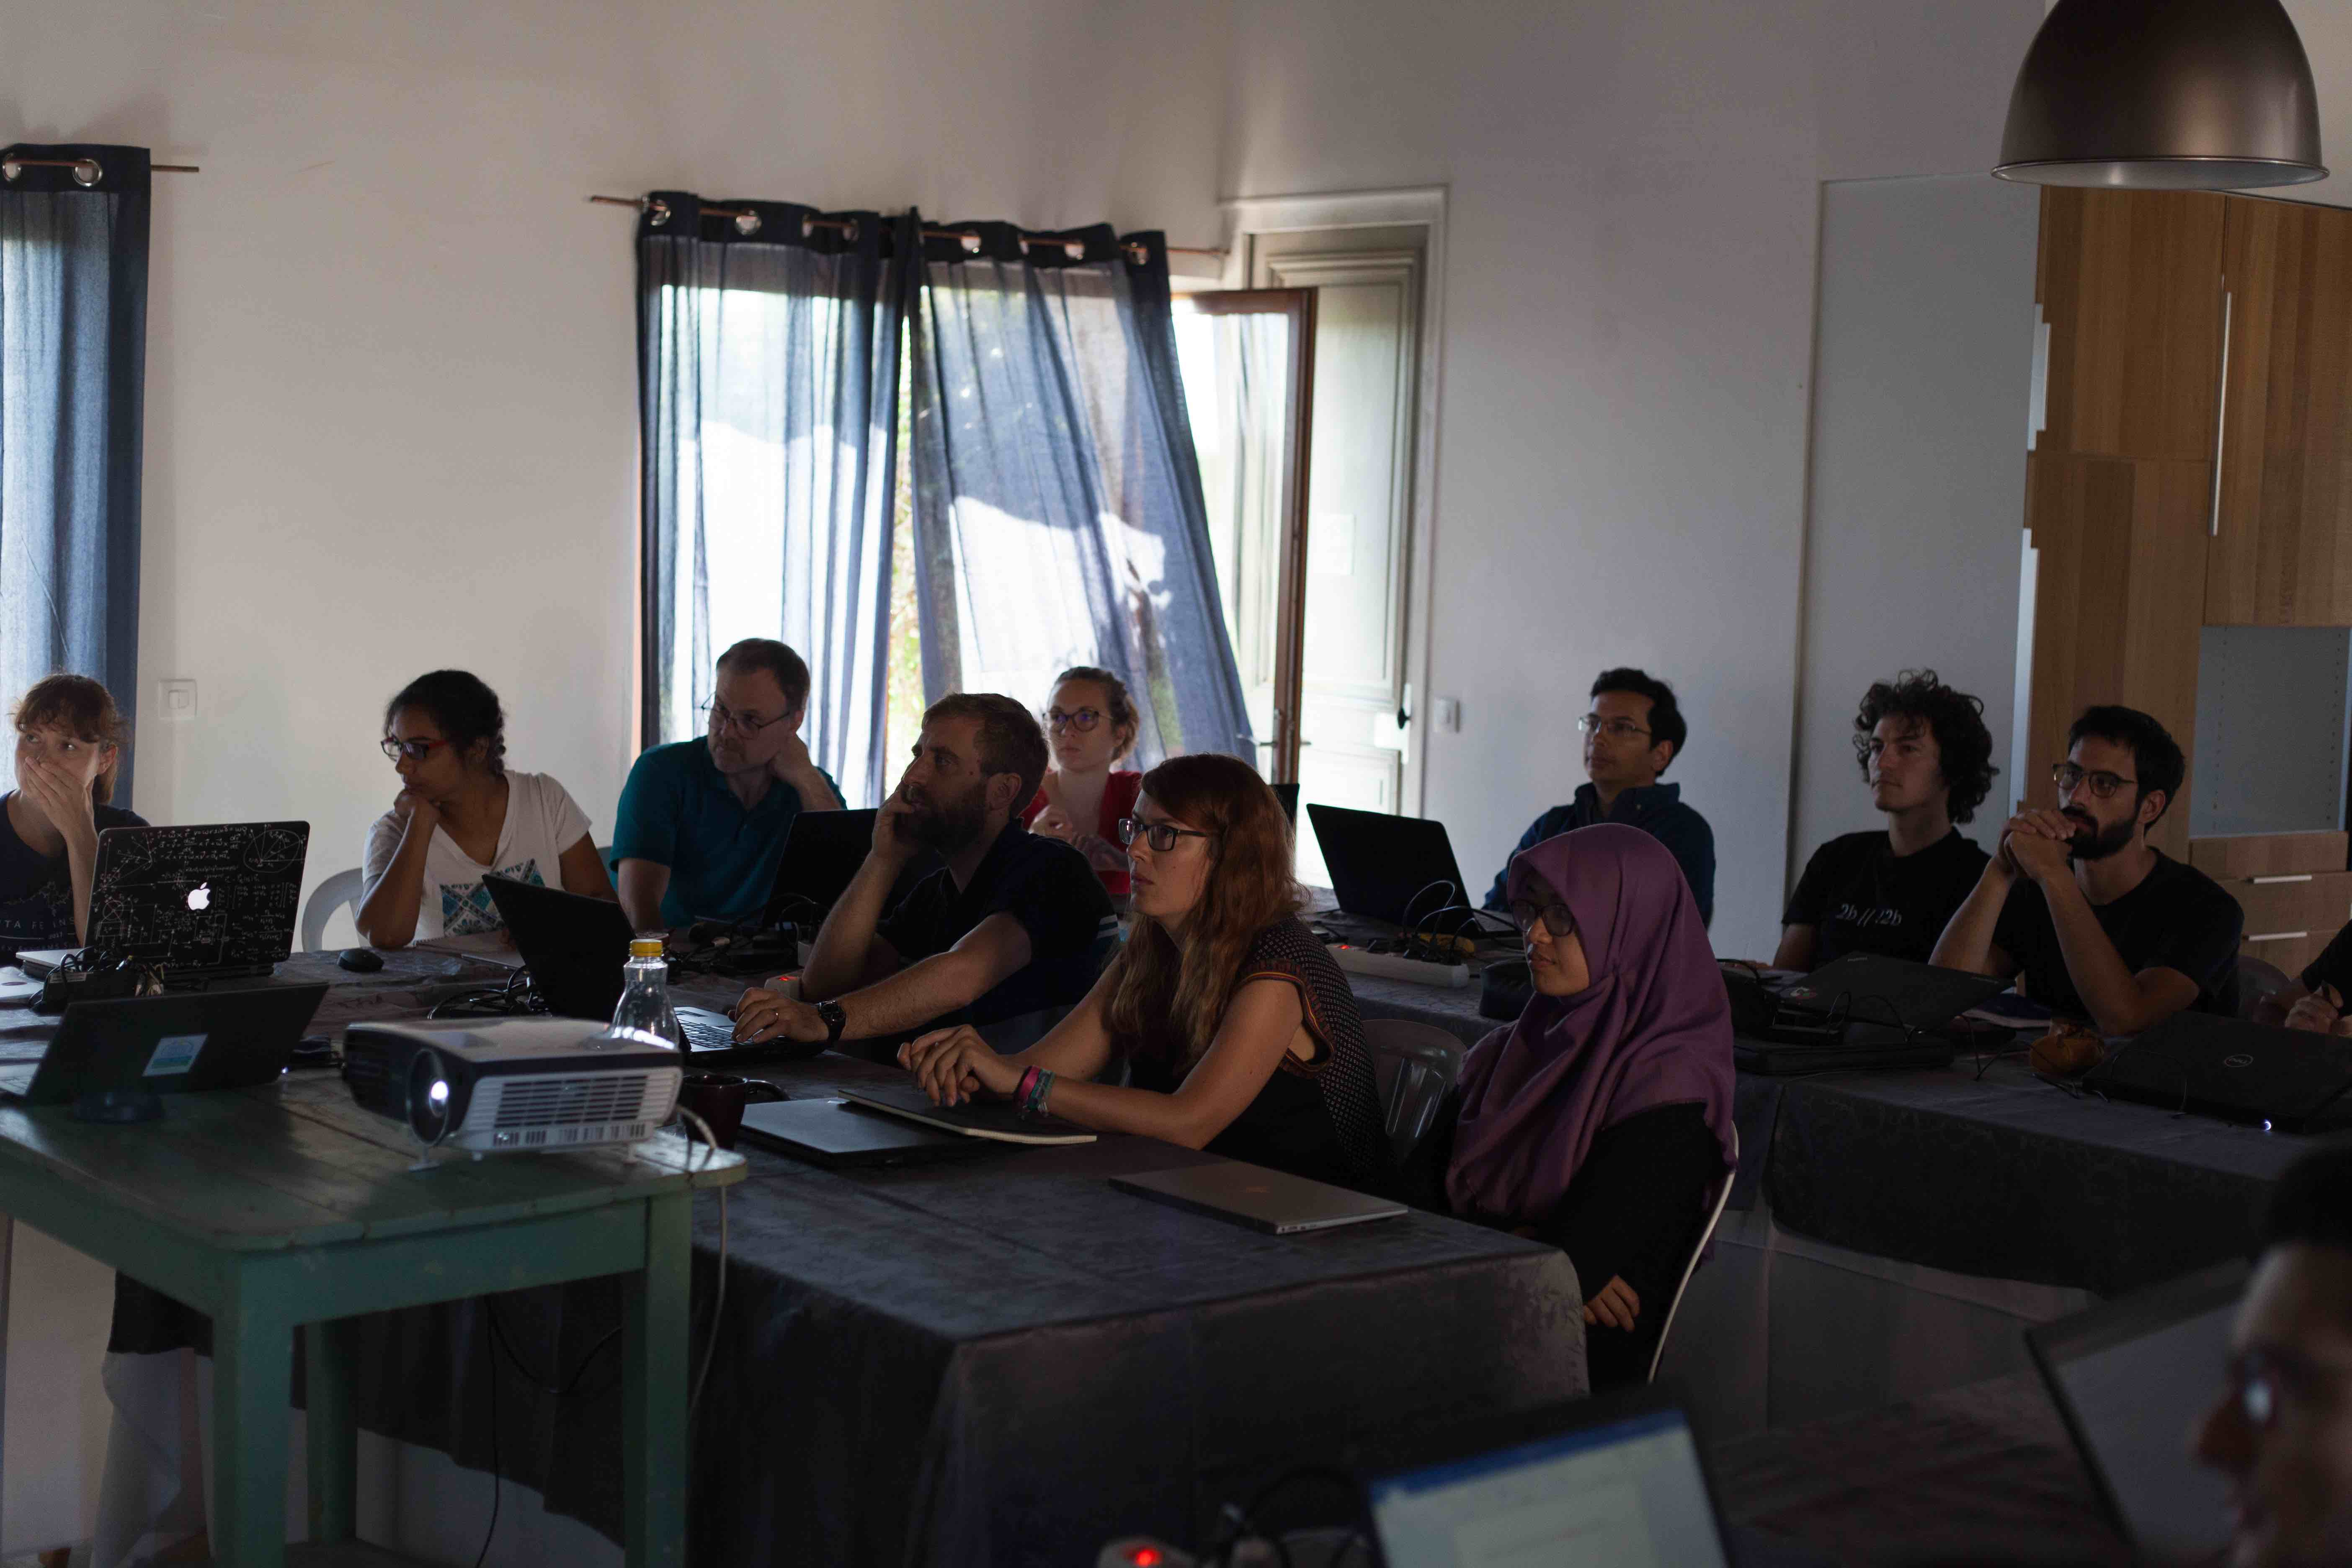
\includegraphics[width=0.58\textwidth]{figures/exmodelo-students_IMG_3206_LR.jpg}\\
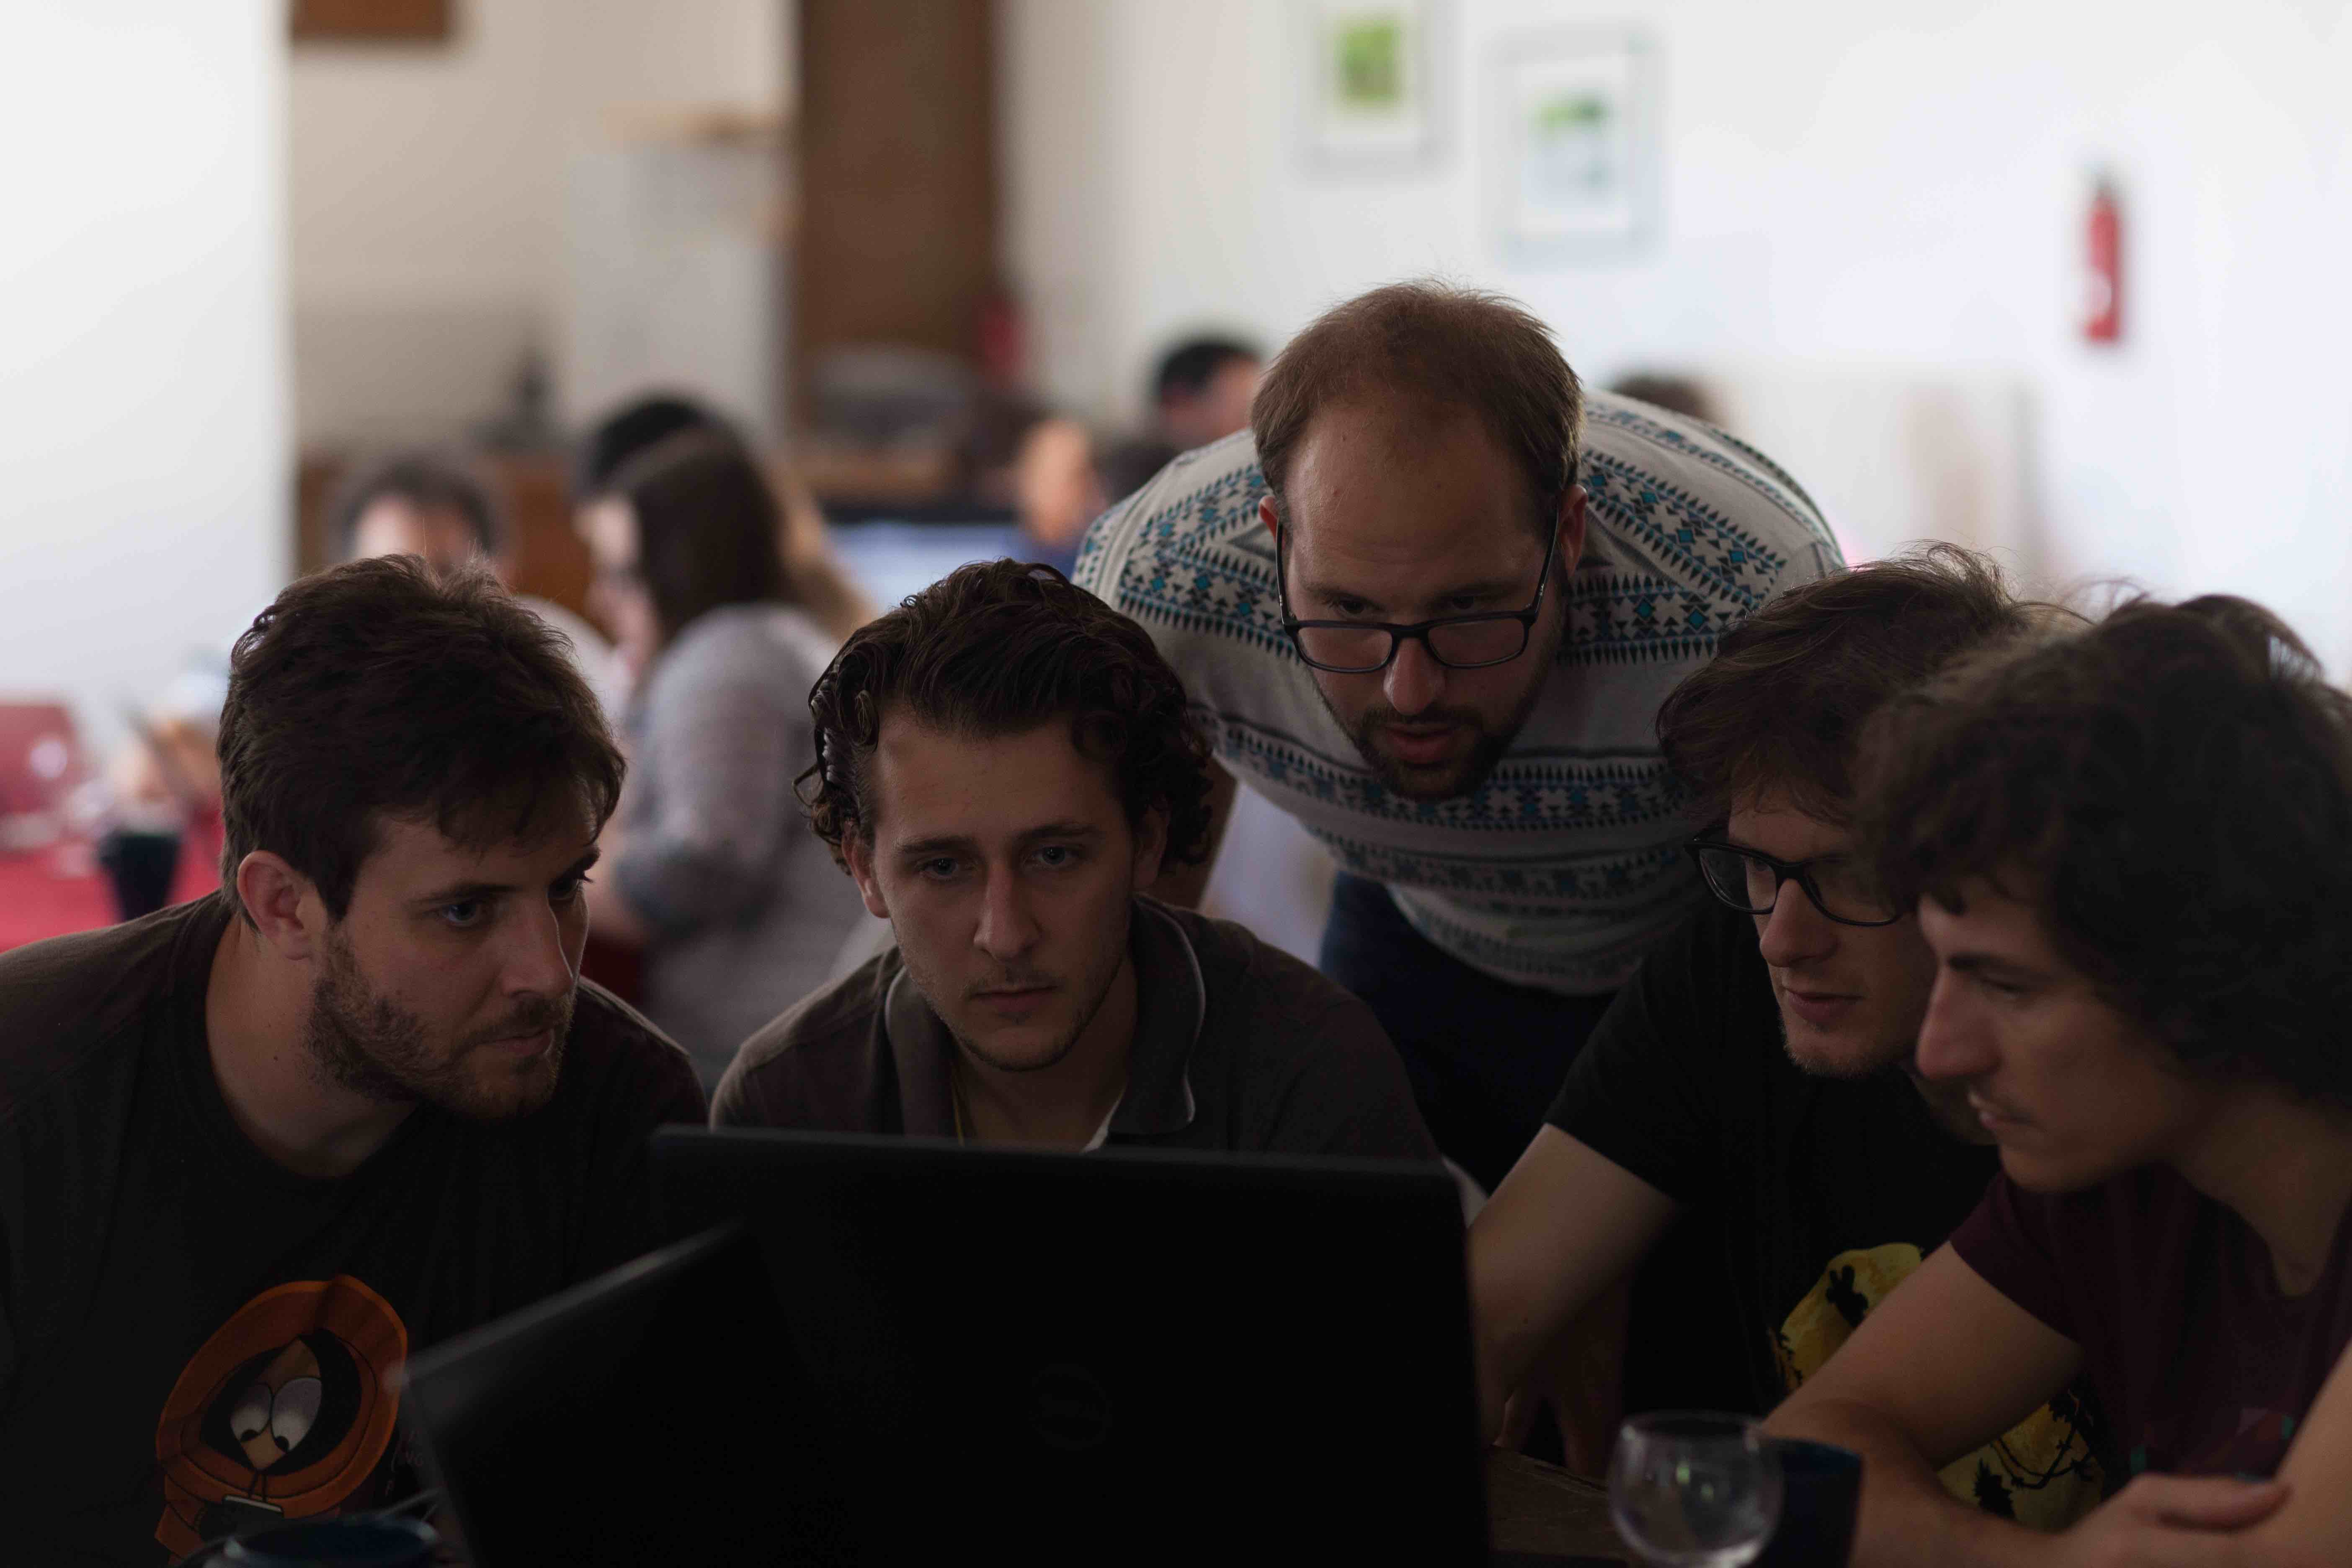
\includegraphics[width=0.58\textwidth]{figures/exmodelo-francois_IMG_3488.jpg}




}



\sframe{... and intensive computation}{

\centering

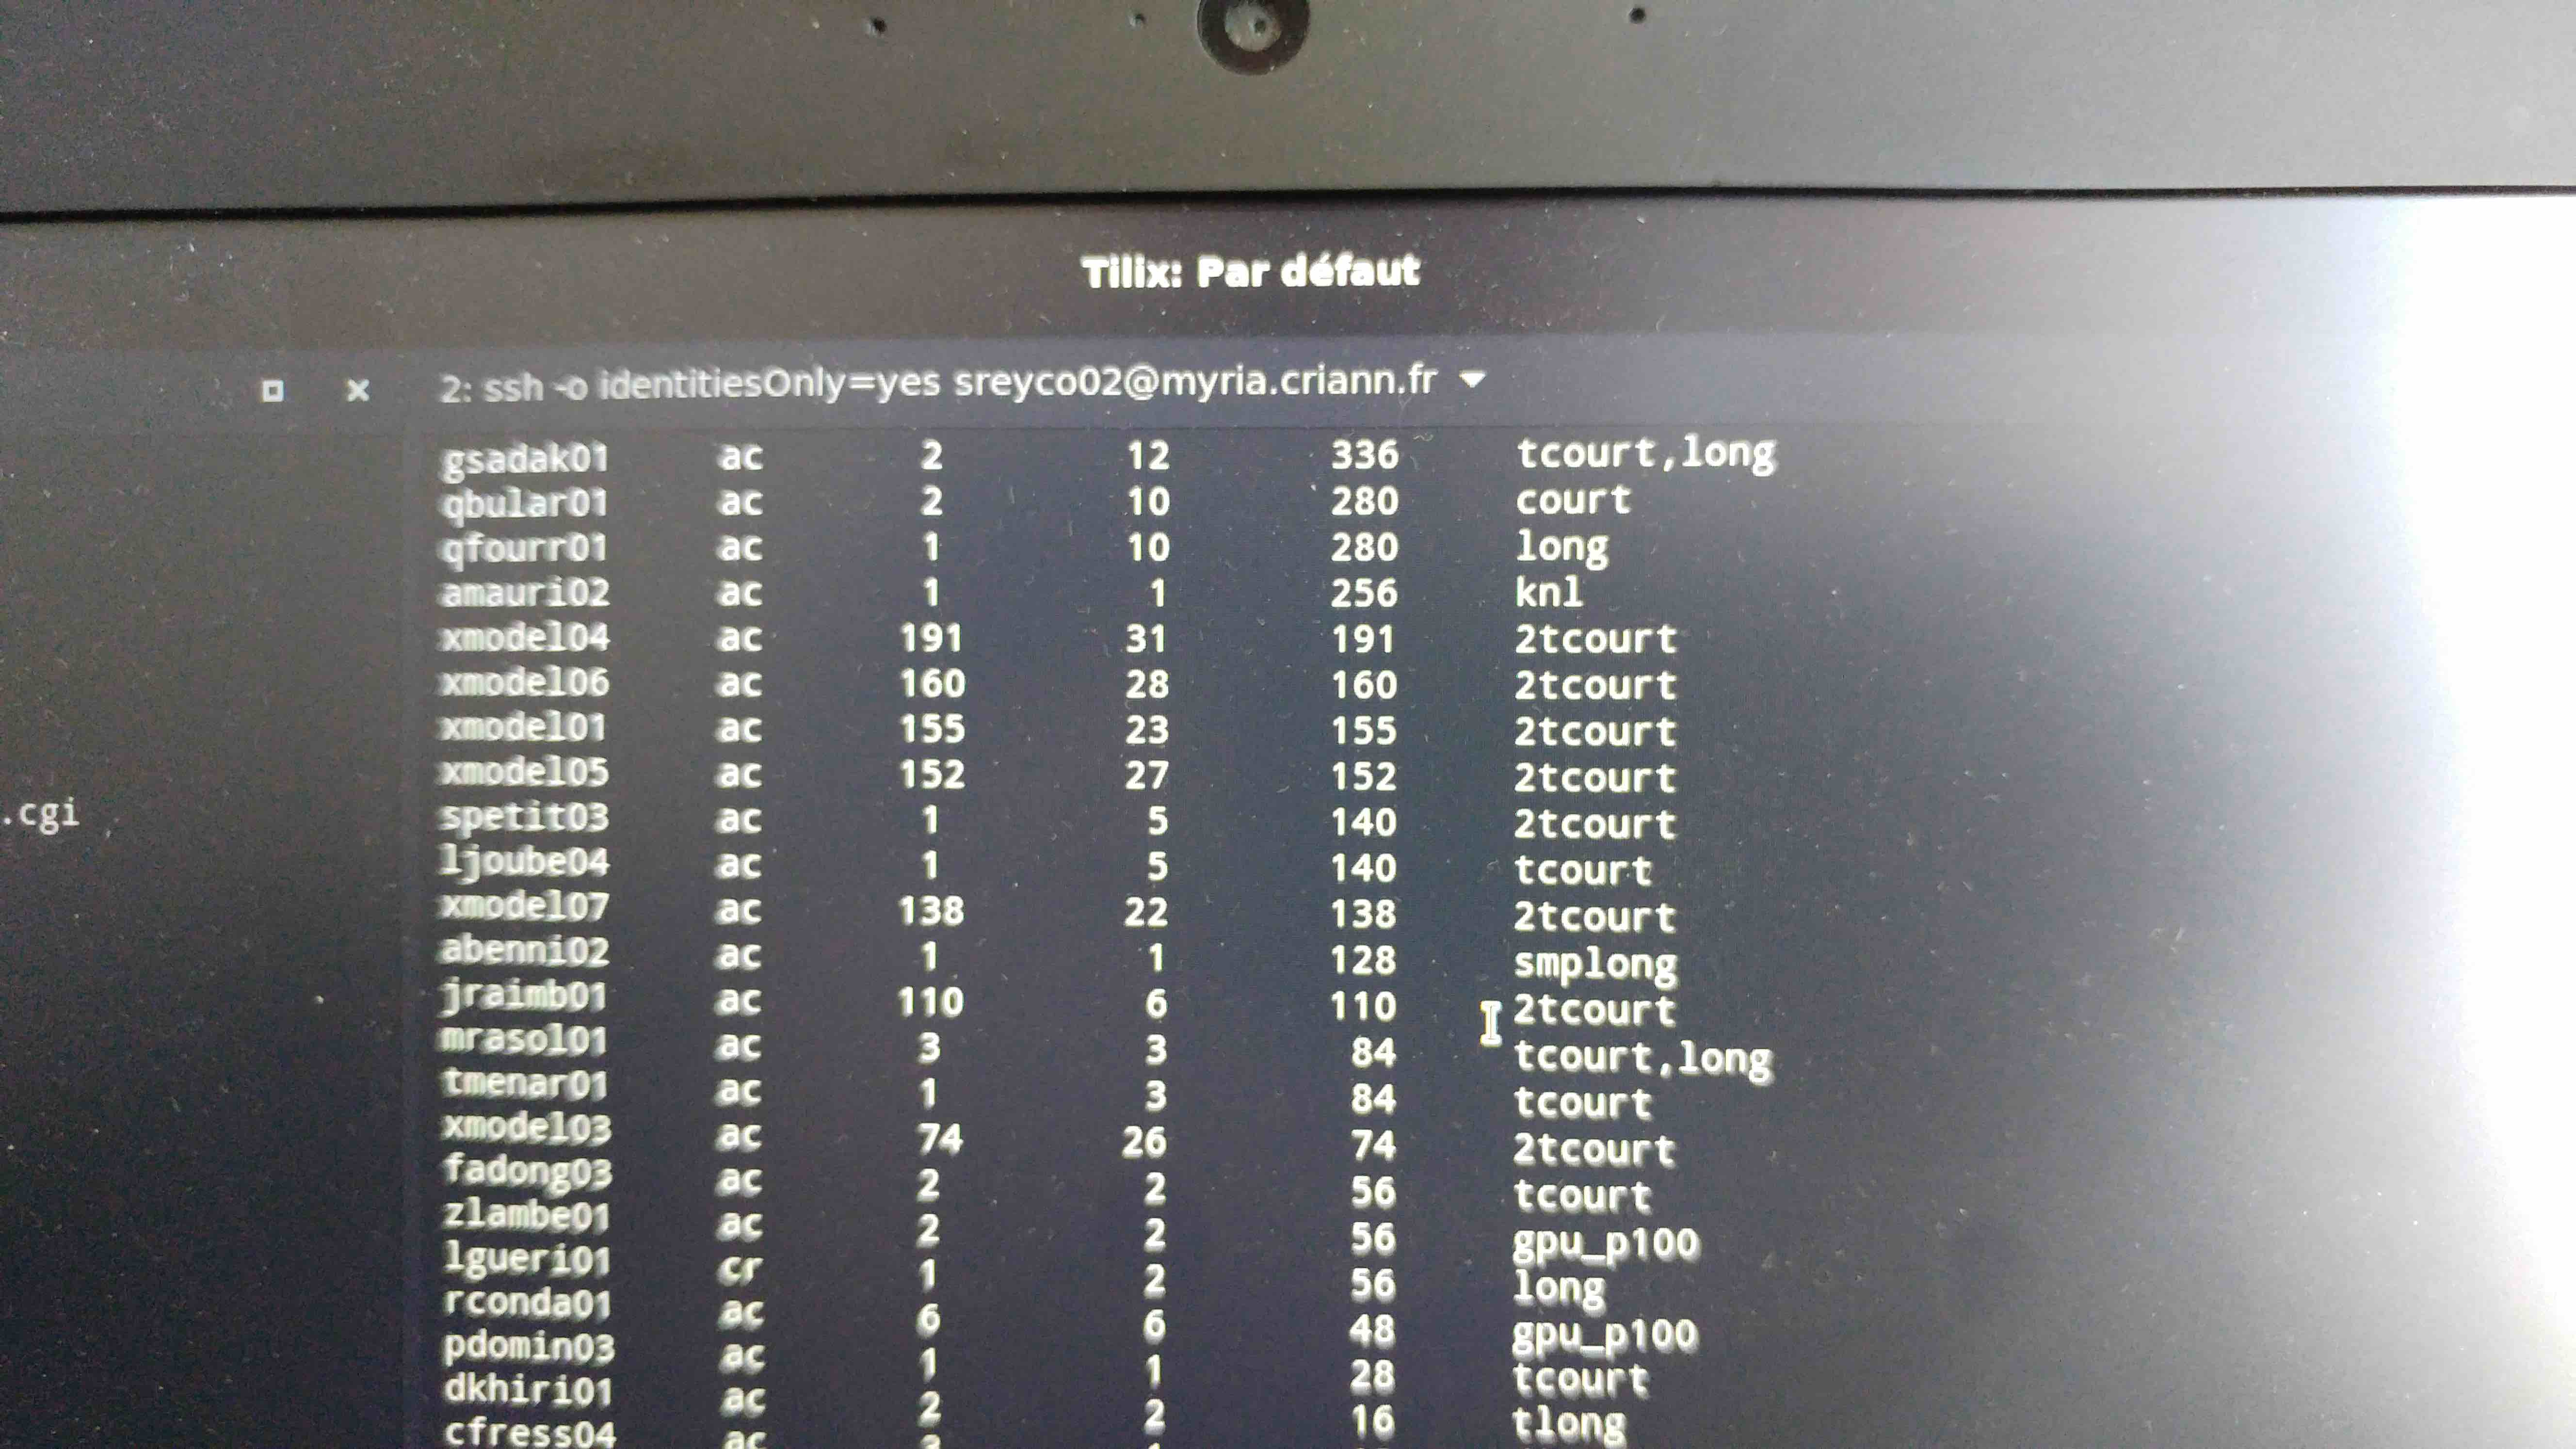
\includegraphics[width=0.58\textwidth]{figures/exmodelo-myria_20190625_123342_LR.jpg}\\
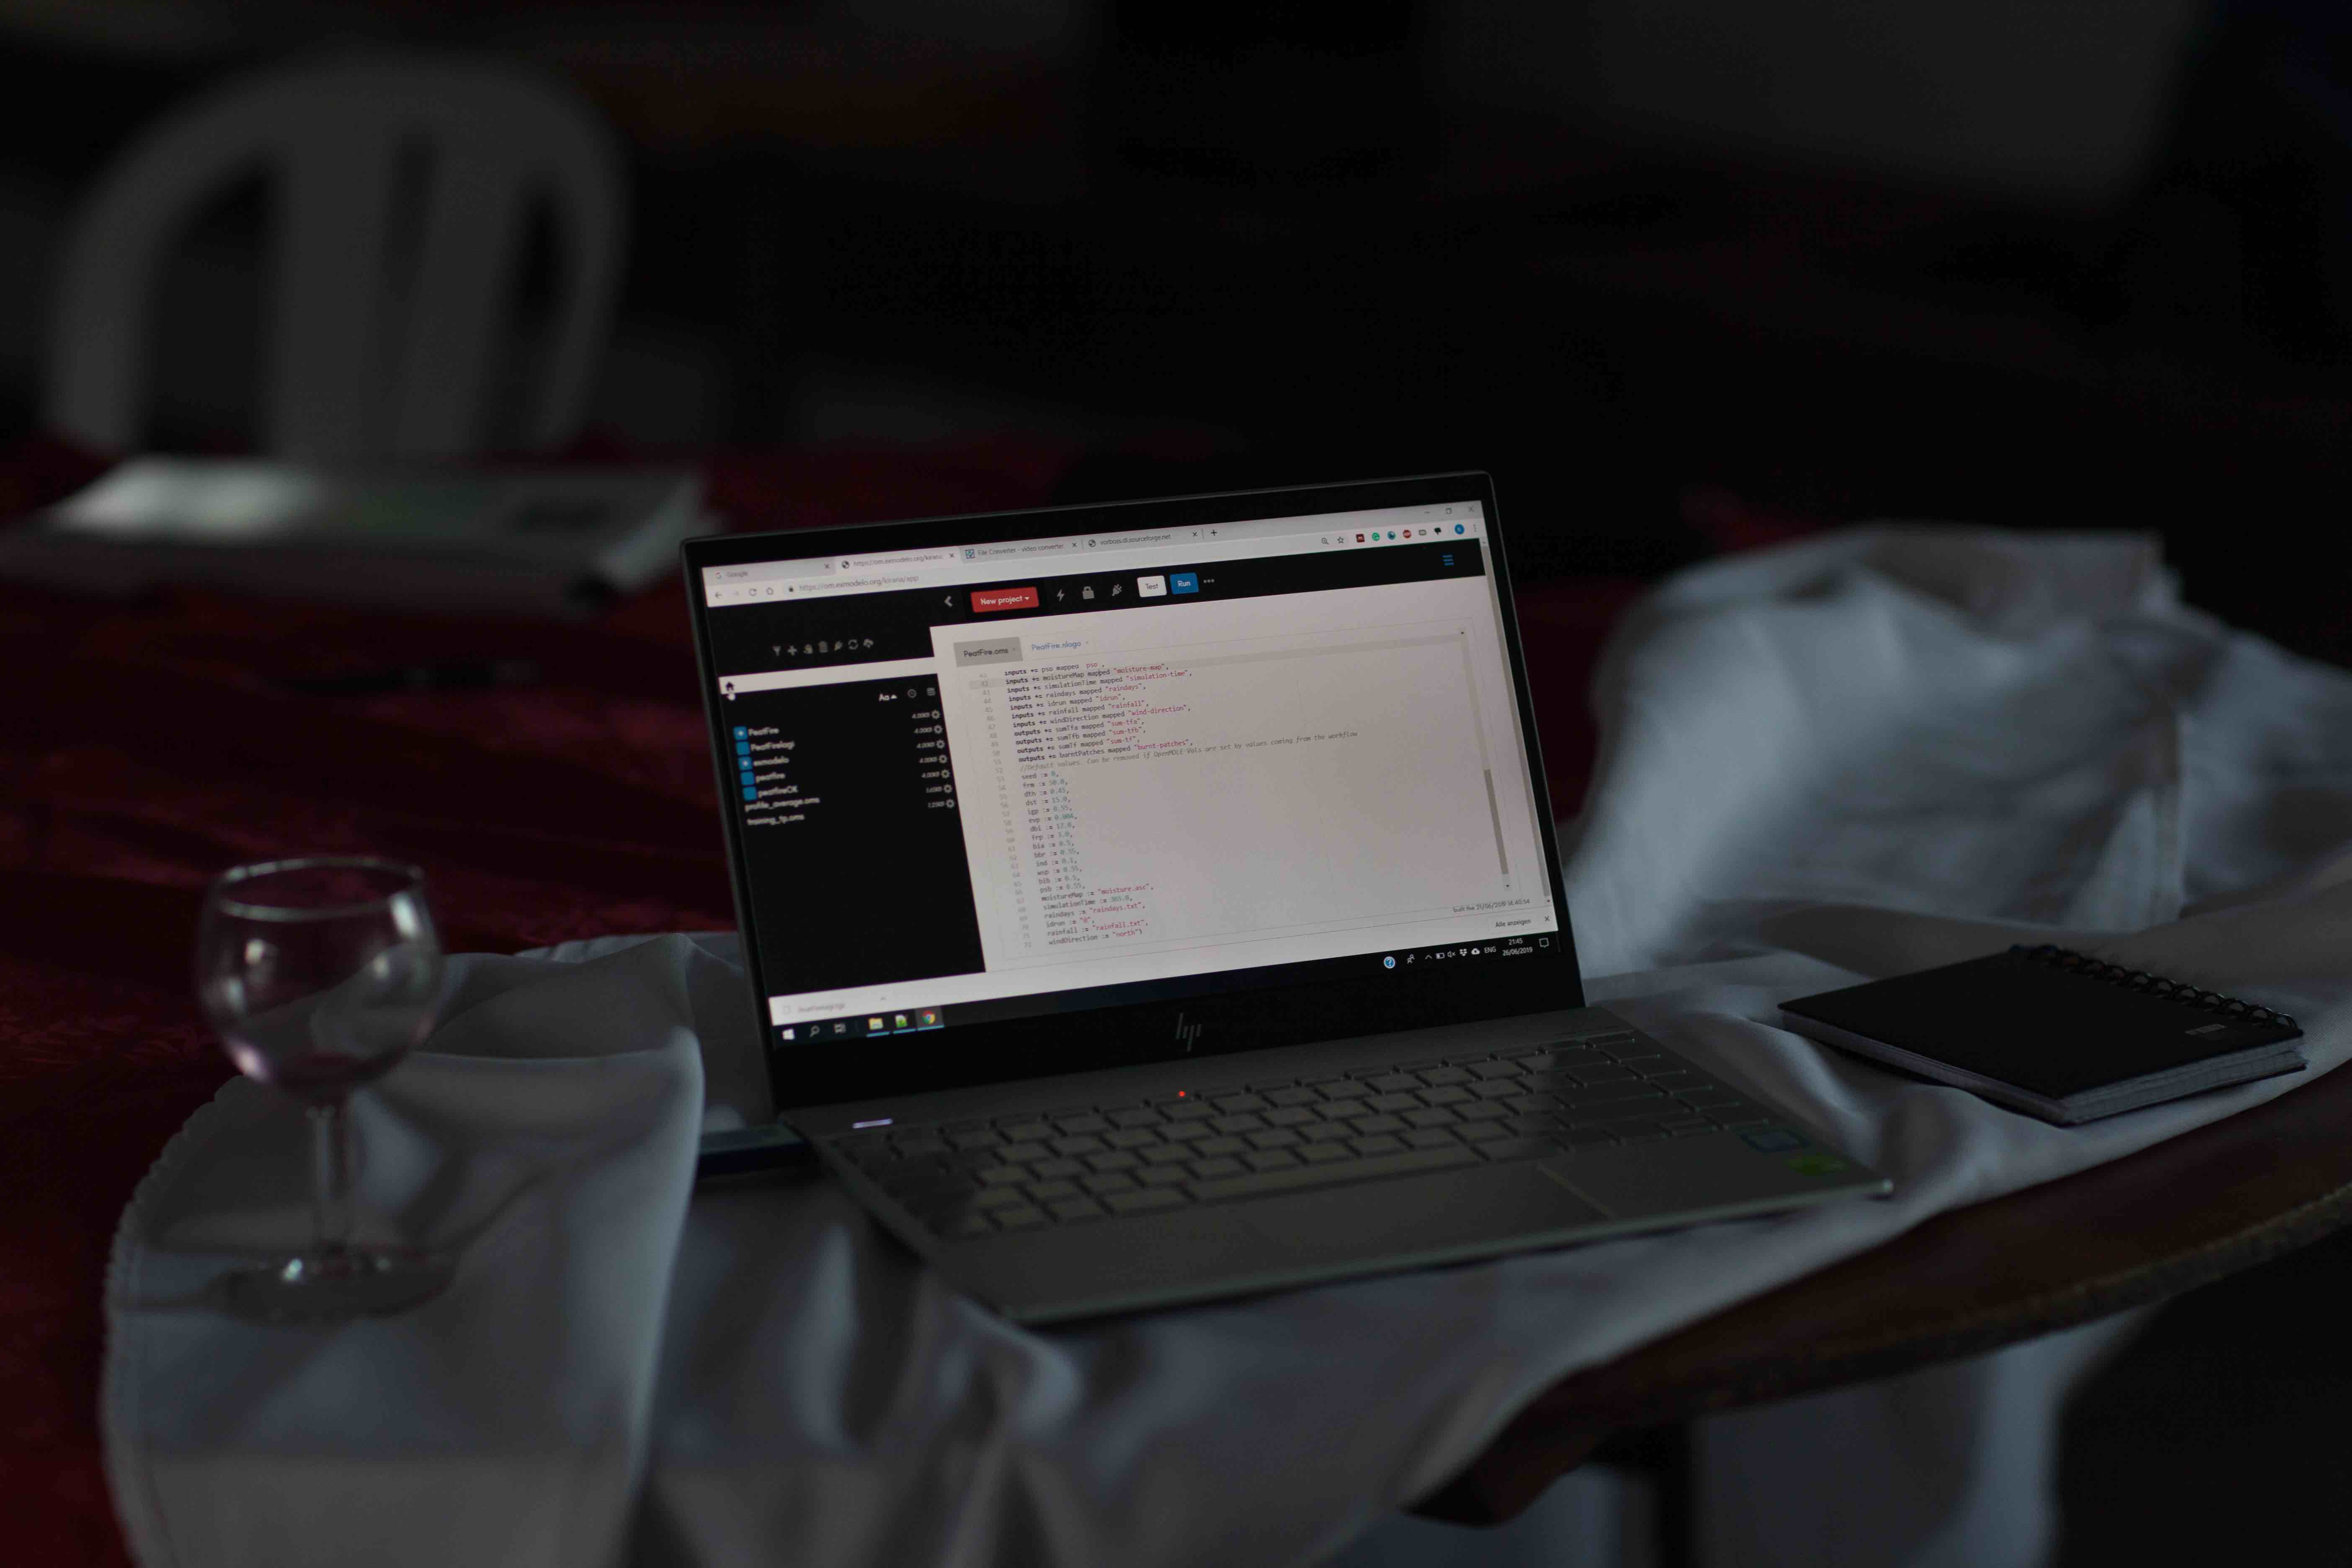
\includegraphics[width=0.58\textwidth]{figures/exmodelo-ordioml_IMG_3786_LR.jpg}

}


\sframe{Model used}{

%We present the iterative exploration and validation protocol developed during the school, with methods of increasing refinement deployed on a toy geosimulation model (spatialized prey-predator agent-based model of a zombie infection, with multi-modeling paradigms to include diverse processes for agent behavior).

% -> global guideline / progression in methods

% - why a zombie model ? : kind of discipline-agnostic [difficulty of interdisciplinary dialogue / integration]

\textit{A common model to present the exploration and validation protocol}

\medskip

$\rightarrow$ modularity and complementarity of aspects

\medskip

$\rightarrow$ possibility of an increased complexity and research questions left open
% possibility of complexification  ? (à la place de increased complexity) 

\bigskip

\textit{A discipline-agnostic model: zombie epidemiology}

\medskip

$\rightarrow$ difficulty of interdisciplinary dialogue

\medskip

$\rightarrow$ agent-based spatial modeling as a natural way to enhance it
% with no relation to a priviledged domain

}



\sframe{An operational model for local Zombie invasion}{

\justify



\begin{center}
%\includegraphics[width=\textwidth]{figures/zombieGUI.png}
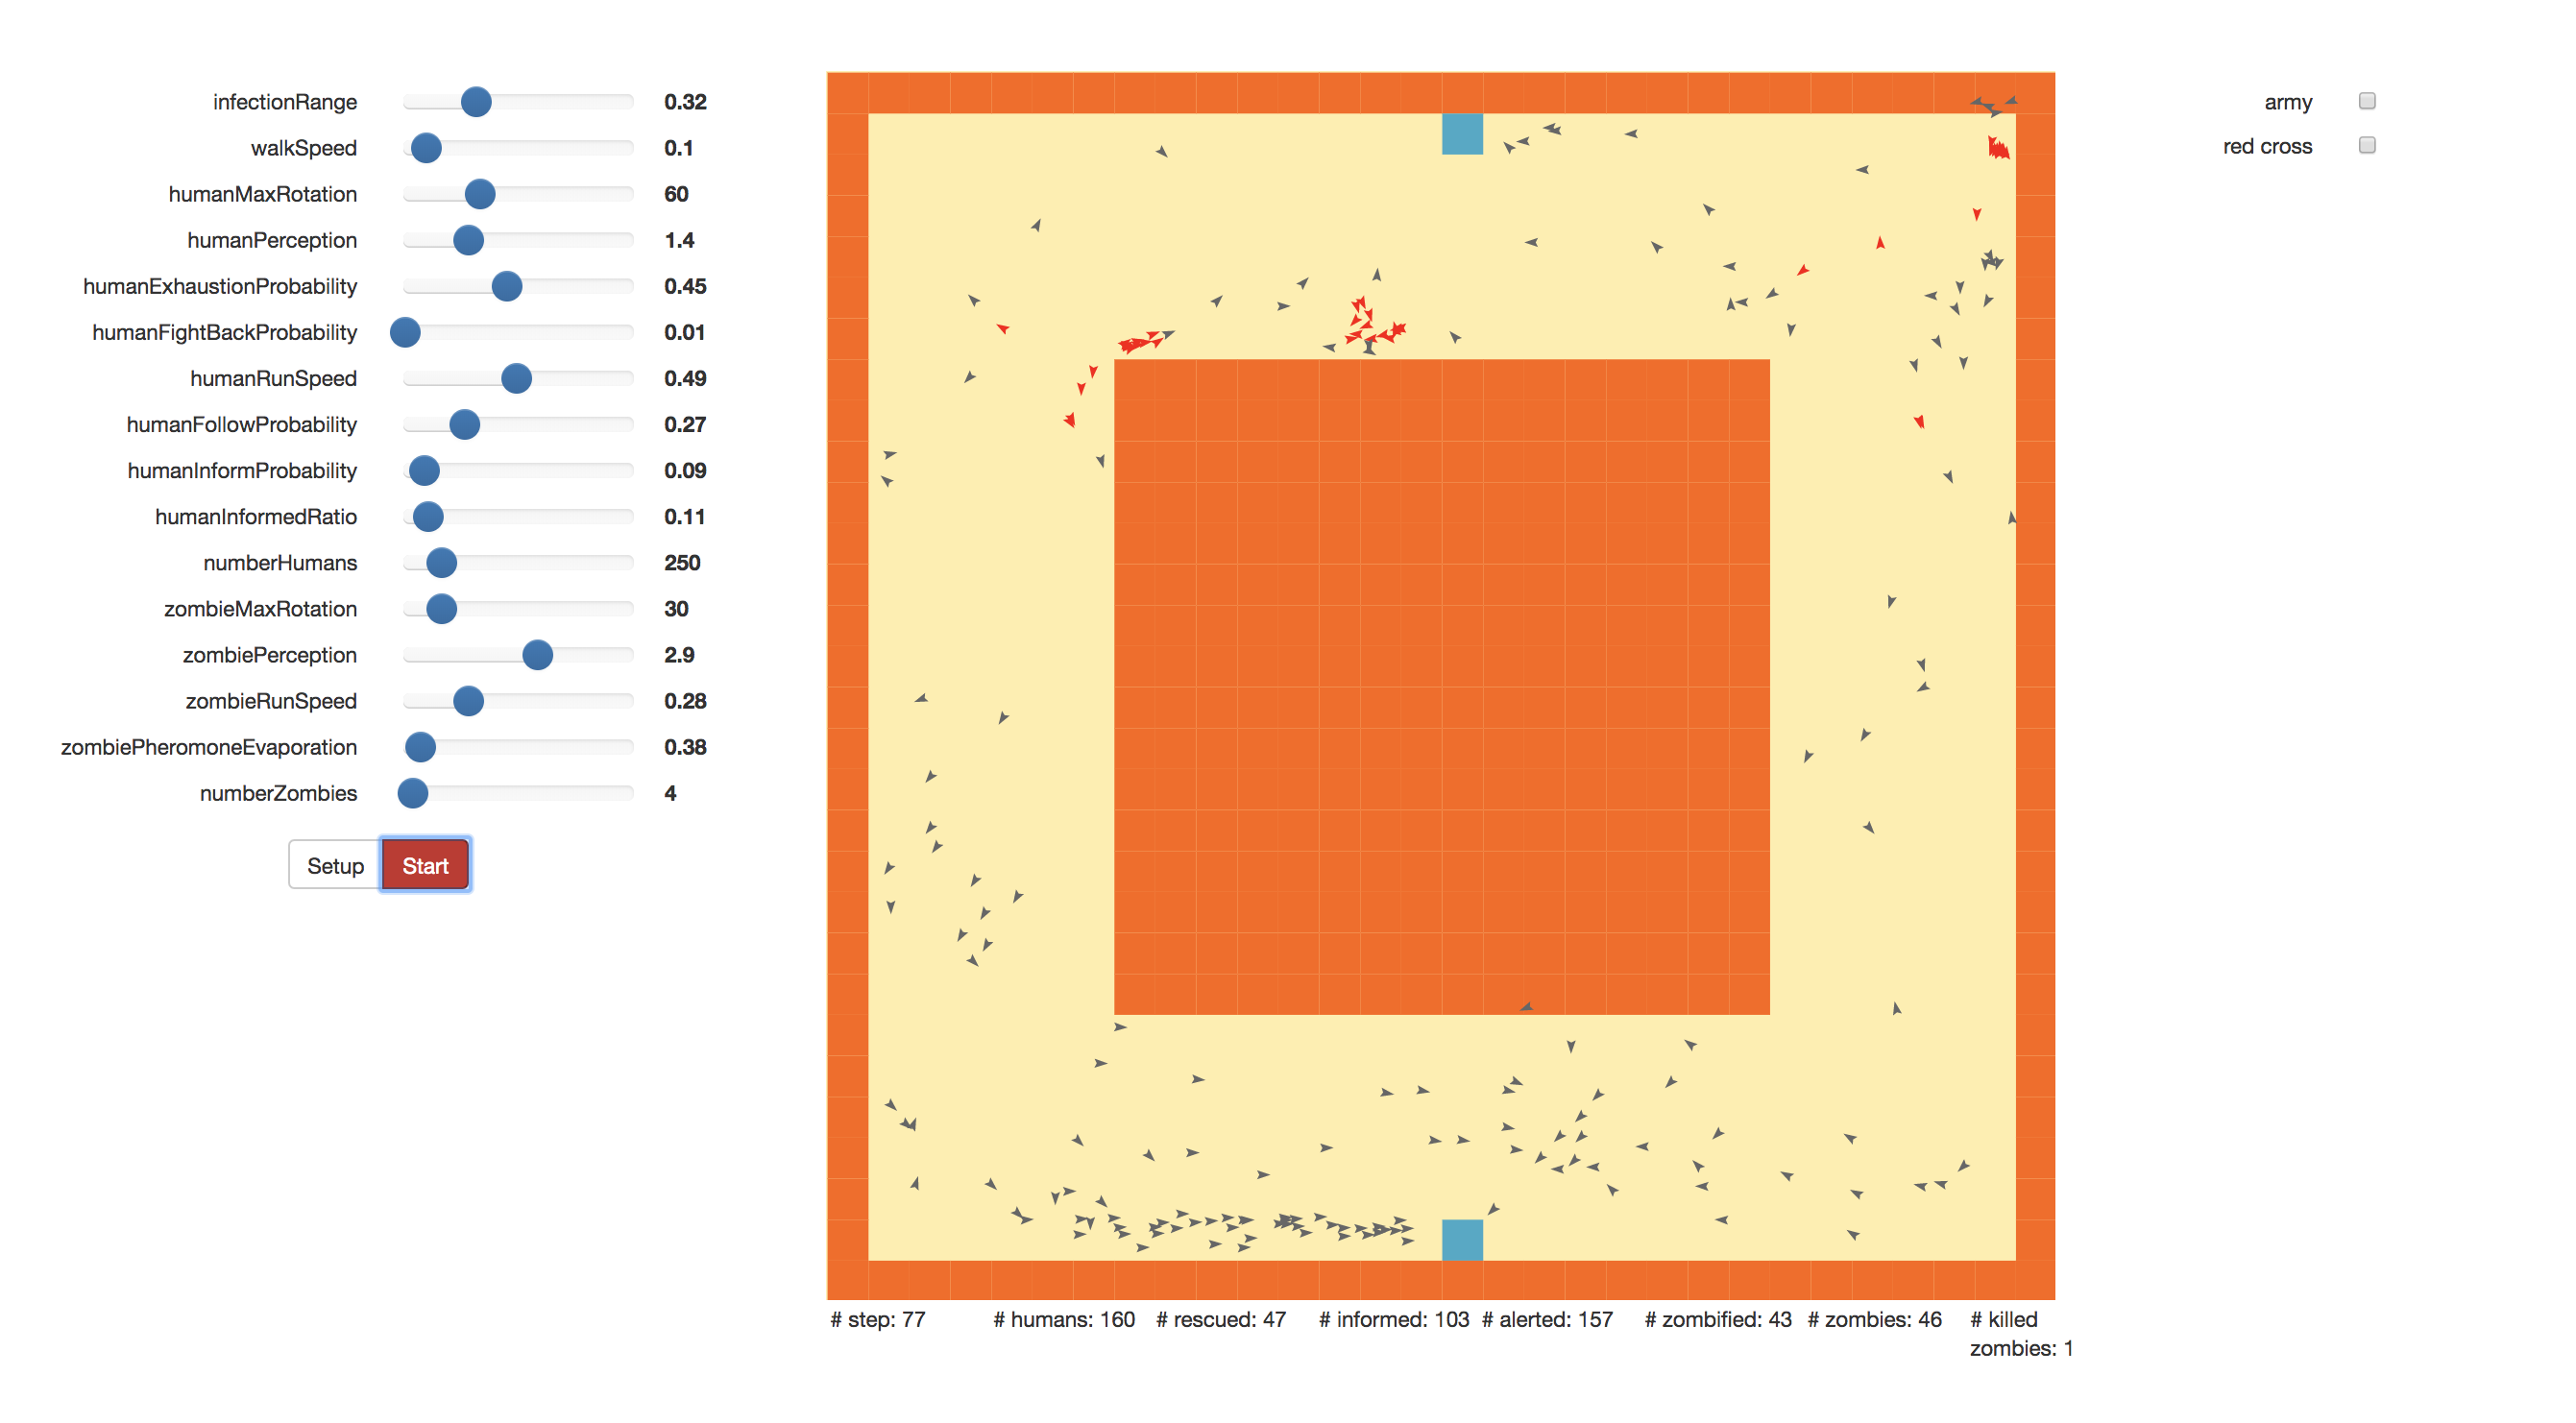
\includegraphics[width=\textwidth]{figures/zombieland_gui.png}
\end{center}

\medskip

\footnotesize

\textit{Local scale agent-based model}

}


\sframe{Agents state machines}{

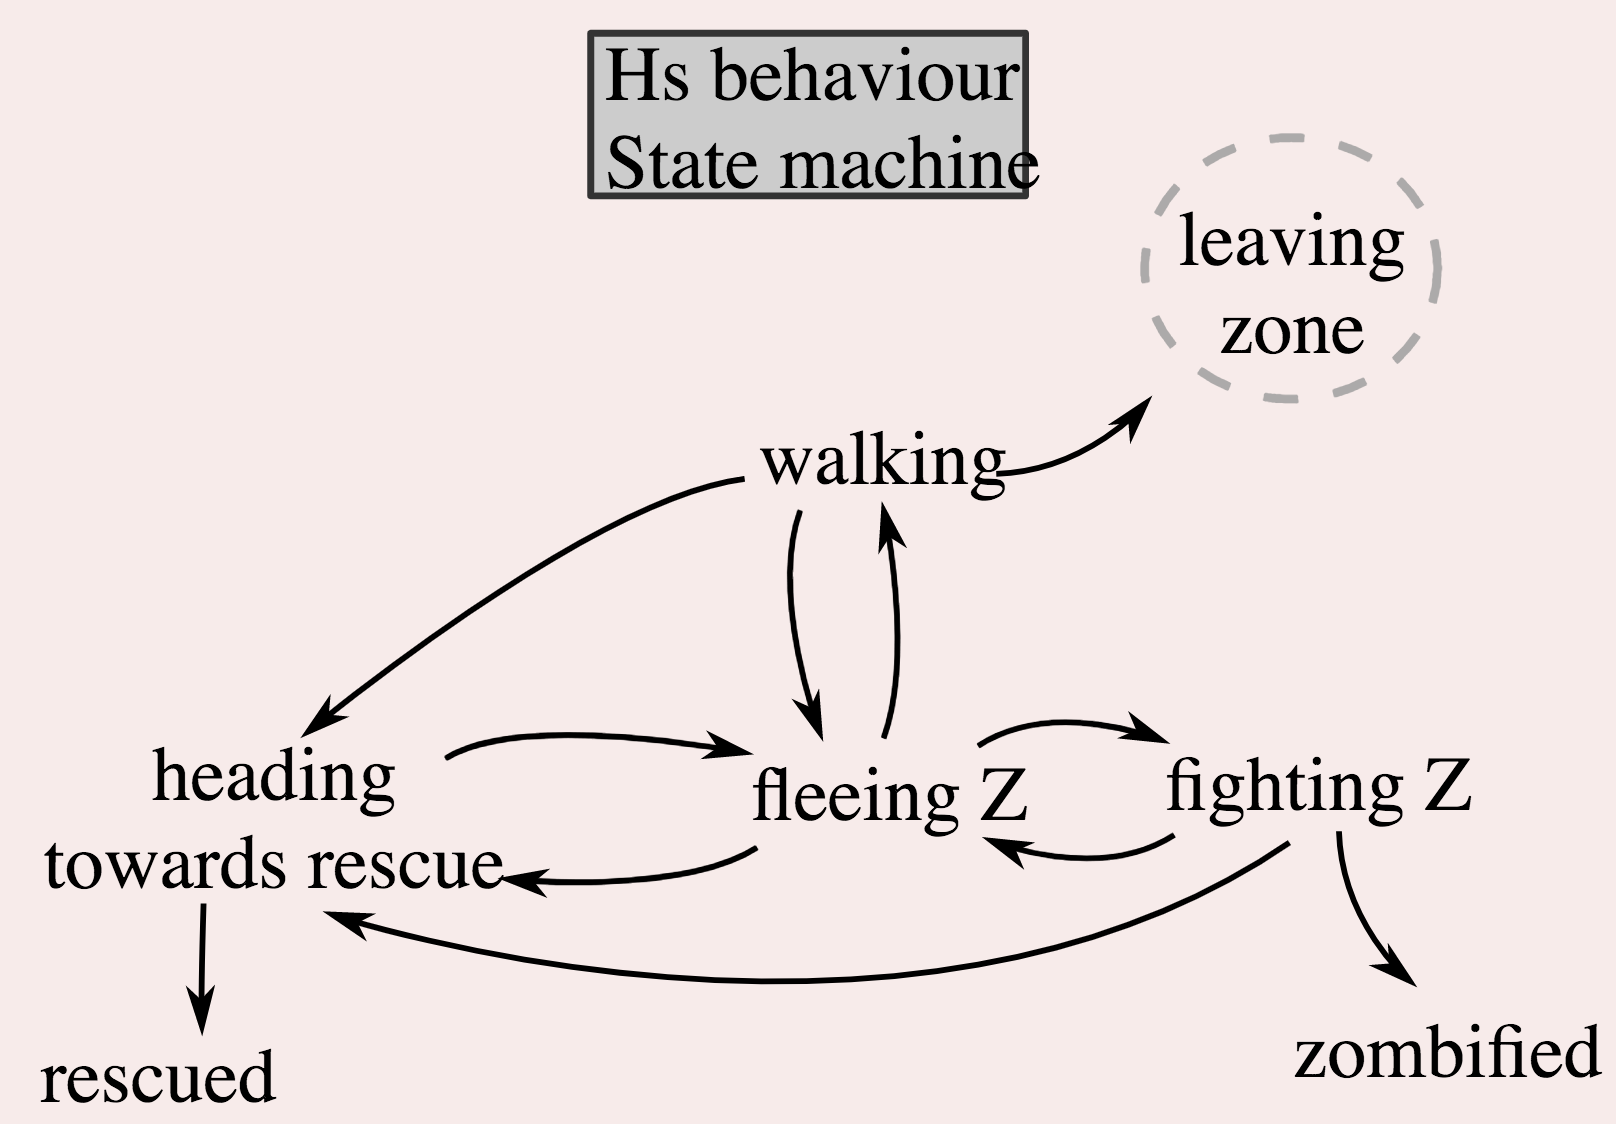
\includegraphics[width=0.51\textwidth]{figures/humanStateMachine.png}\hspace{0.2cm}
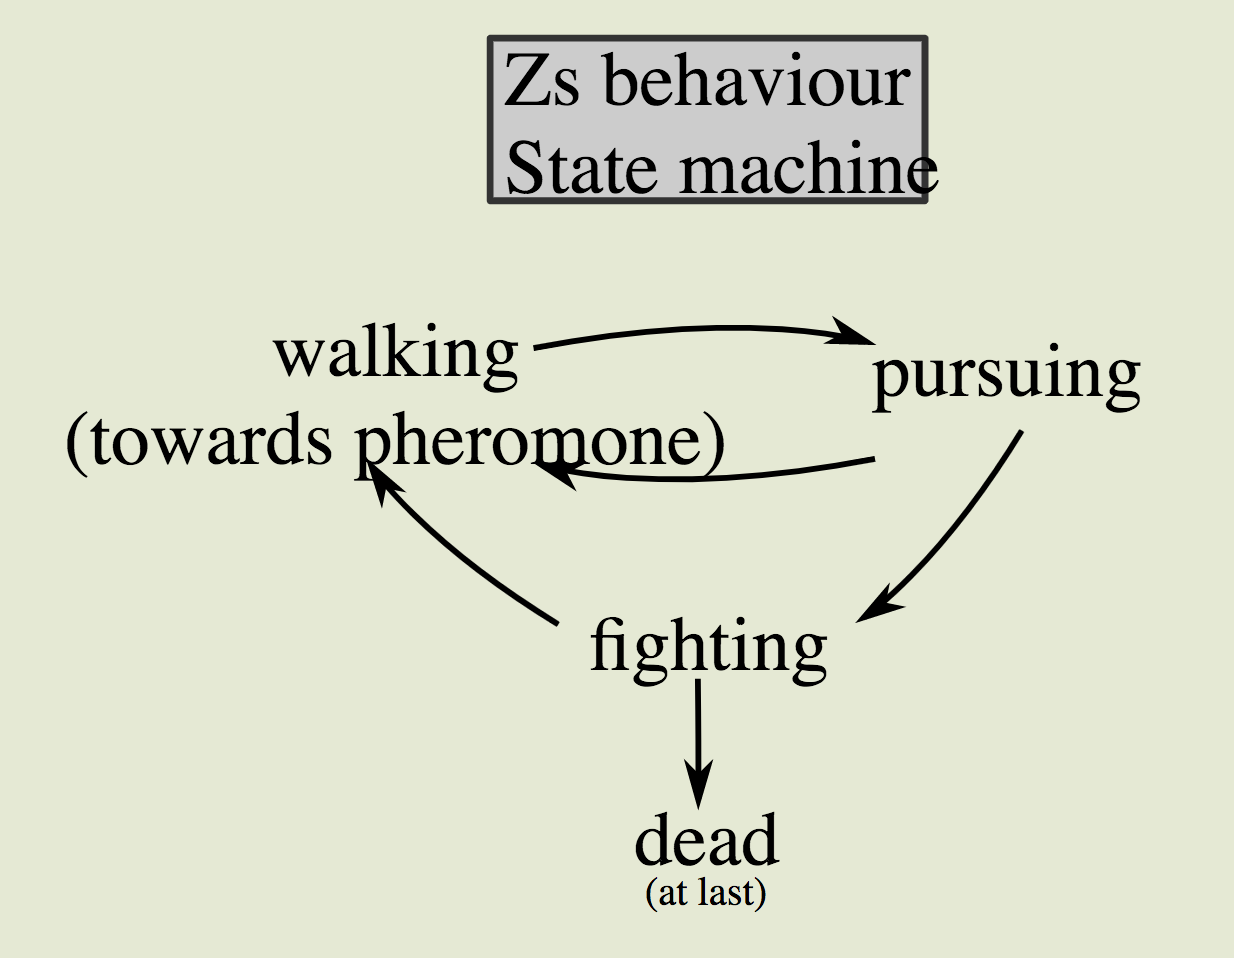
\includegraphics[width=0.46\textwidth]{figures/zombieStateMachine.png}

% launch simu https://om.exmodelo.org/coop/

}




\sframe{Sensitivity analysis}{

% First, we illustrate classical sensitivity analysis methods (stochasticity, design of experiments, global sensitivity indices)

%\textit{Sensitivity analysis: stochasticity, Design of Experiments, sensitivity indices}

\textbf{\textit{Design of Experiments}}


\begin{mdframed}

\begin{columns}
	\begin{column}{0.2\linewidth}
	
	\bigskip
	\bigskip
	
	One factor at a time
	
	\medskip
	
	Complete plan
	
	\medskip
	
	LHS/Sobol
		
	\end{column}
	\begin{column}{0.2\linewidth}
		
		\textbf{Coverage}
		
		\bigskip
		
		{\textcolor{red}
		\xmark
		}
		
		\medskip
		
		{\textcolor{green}
		\cmark
		}
		
		\medskip
		
		{\textcolor{green}
		\cmark
		}
			
	\end{column}
	
	\begin{column}{0.25\linewidth}
		
		\textbf{Interpretability}
		
		\bigskip
		
		{\textcolor{green}
		\cmark
		}
		
		\medskip
		
		{\textcolor{green}
		\cmark
		}
		
		\medskip
		
		{\textcolor{red}
		\xmark
		}	
	\end{column}
	
	\begin{column}{0.2\linewidth}
		
		\textbf{Budget}
		
		\bigskip
		
		{\textcolor{green}
		\cmark
		}
		
		\medskip
		
		{\textcolor{red}
		\xmark
		}
		
		\medskip
		
		{\textcolor{green}
		\cmark
		}	
	\end{column}

	
	
	
\end{columns}

	
\end{mdframed}

\bigskip

\textbf{\textit{Sensitivity analysis}}

\begin{mdframed}
	\begin{columns}
	\begin{column}{0.2\linewidth}
	
	\bigskip
	\bigskip
	
	Morris
	
	\medskip
	
	Saltelli
	

		
	\end{column}
	\begin{column}{0.2\linewidth}
		
		\textbf{Coverage}
		
		\bigskip
		
		{\textcolor{red}
		\xmark
		}
		
		\medskip
		
		{\textcolor{green}
		\cmark
		}
		
	
			
	\end{column}
	
	\begin{column}{0.25\linewidth}
		
		\textbf{Interpretability}
		
		\bigskip
		
		{\textcolor{green}
		\cmark
		}
		
		\medskip
		
		{\textcolor{green}
		\cmark
		}
			
	\end{column}
	
	\begin{column}{0.2\linewidth}
		
		\textbf{Budget}
		
		\bigskip
		
		{\textcolor{green}
		\cmark
		}
		
		\medskip
		
		{\textcolor{red}
		\xmark
		}
			
	\end{column}

	
	
	
\end{columns}
	
\end{mdframed}



}



\sframe{Example: Morris sensitivity}{

\textit{Syntax of a sensitivity analysis method in OpenMOLE}

\bigskip

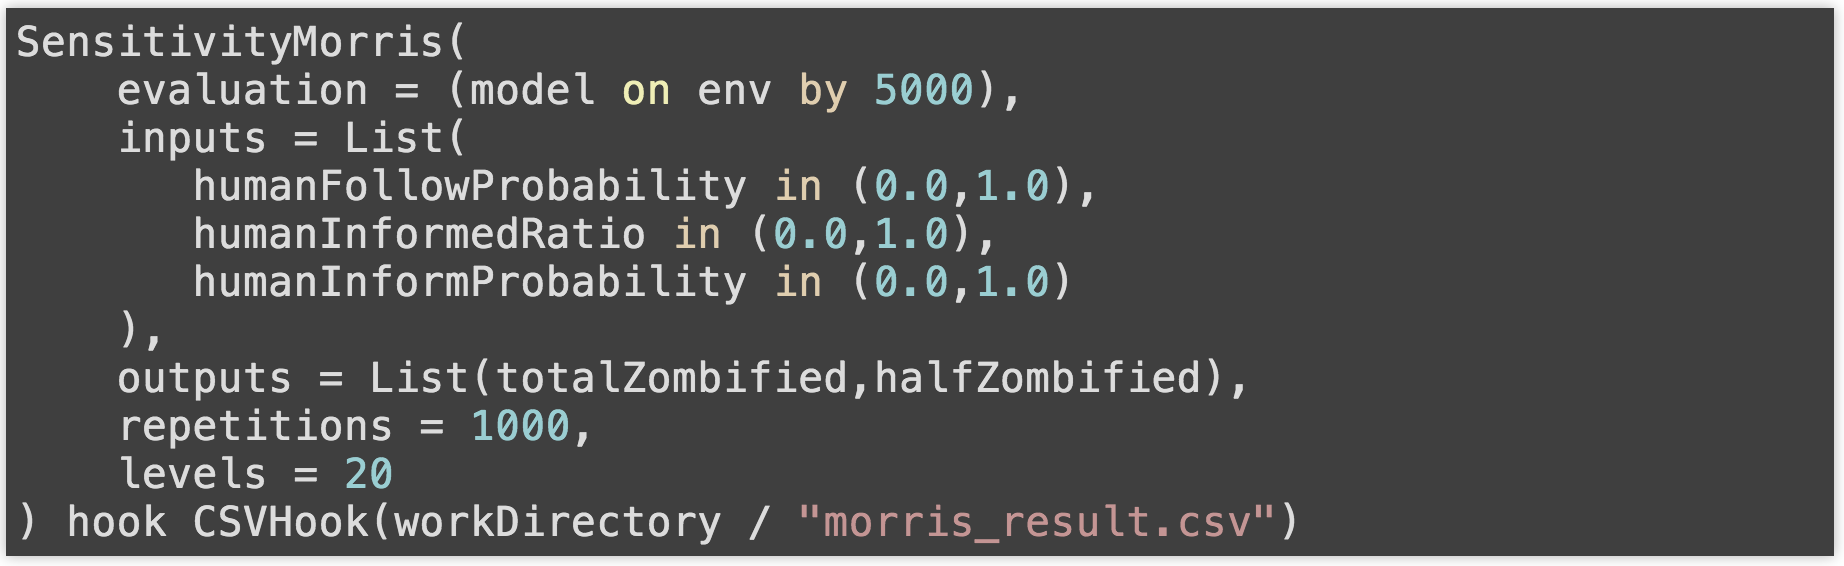
\includegraphics[width=\textwidth]{figures/morris_code.png}

\bigskip

$\rightarrow$ \textbf{Practice for students at eXModelo: } explore the script \texttt{morris.oms}, comment the results obtained with a large-scale experiment \texttt{morrisresults}

}



\sframe{Advanced methods}{

%, and then specific methods to study spatial configuration sensitivity, evolutionary computation methods for calibration and diversity search, and Bayesian calibration methods.

\textbf{Calibration}: Evolutionary (GA) and Bayesian (ABC) methods 

\bigskip

\textbf{Diversity Search}: "look for the variety of obtainable patterns in output space" 
\bigskip

\textbf{Origin Search}: "look for the input that produce a given pattern in output space"


}


\sframe{Advanced methods: spatial sensitivity}{

\textit{A specific focus on spatial aspects: built-in spatial sensitivity analysis library }

%\begin{itemize}
%    \item Moran's I : spatial autocorrelation at a given range
%    \item Ripley's K : points clustering level
%    \item Geographically Weighted Regression
%\end{itemize}
%\bigskip

%e.g. Zombie invasion urban guerilla design : which spatial organization impedes the epidemics ?  

\bigskip

Example: generators of synthetic urban districts \cite{doi10.1162isala00159}

\medskip

\centering

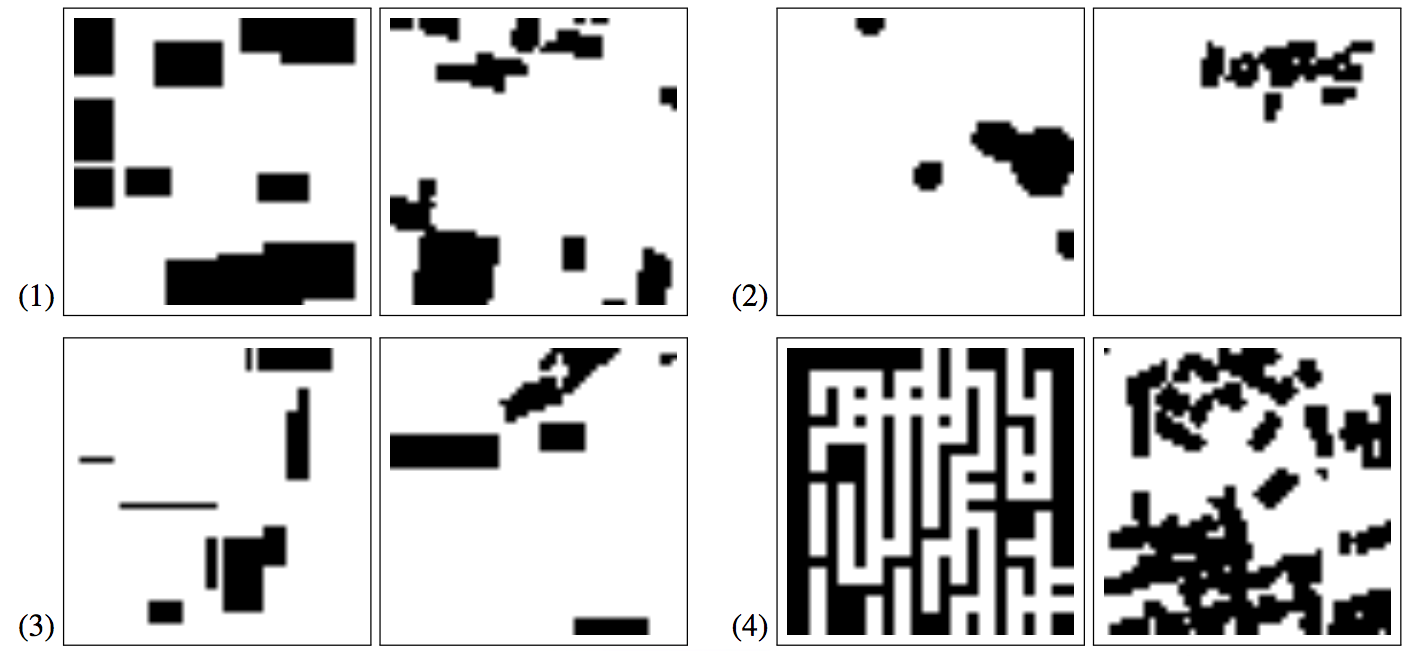
\includegraphics[width=\textwidth]{figures/spatialsens_calib.png}




}

\sframe{Modifying the world in the Zombie model}{

\centering

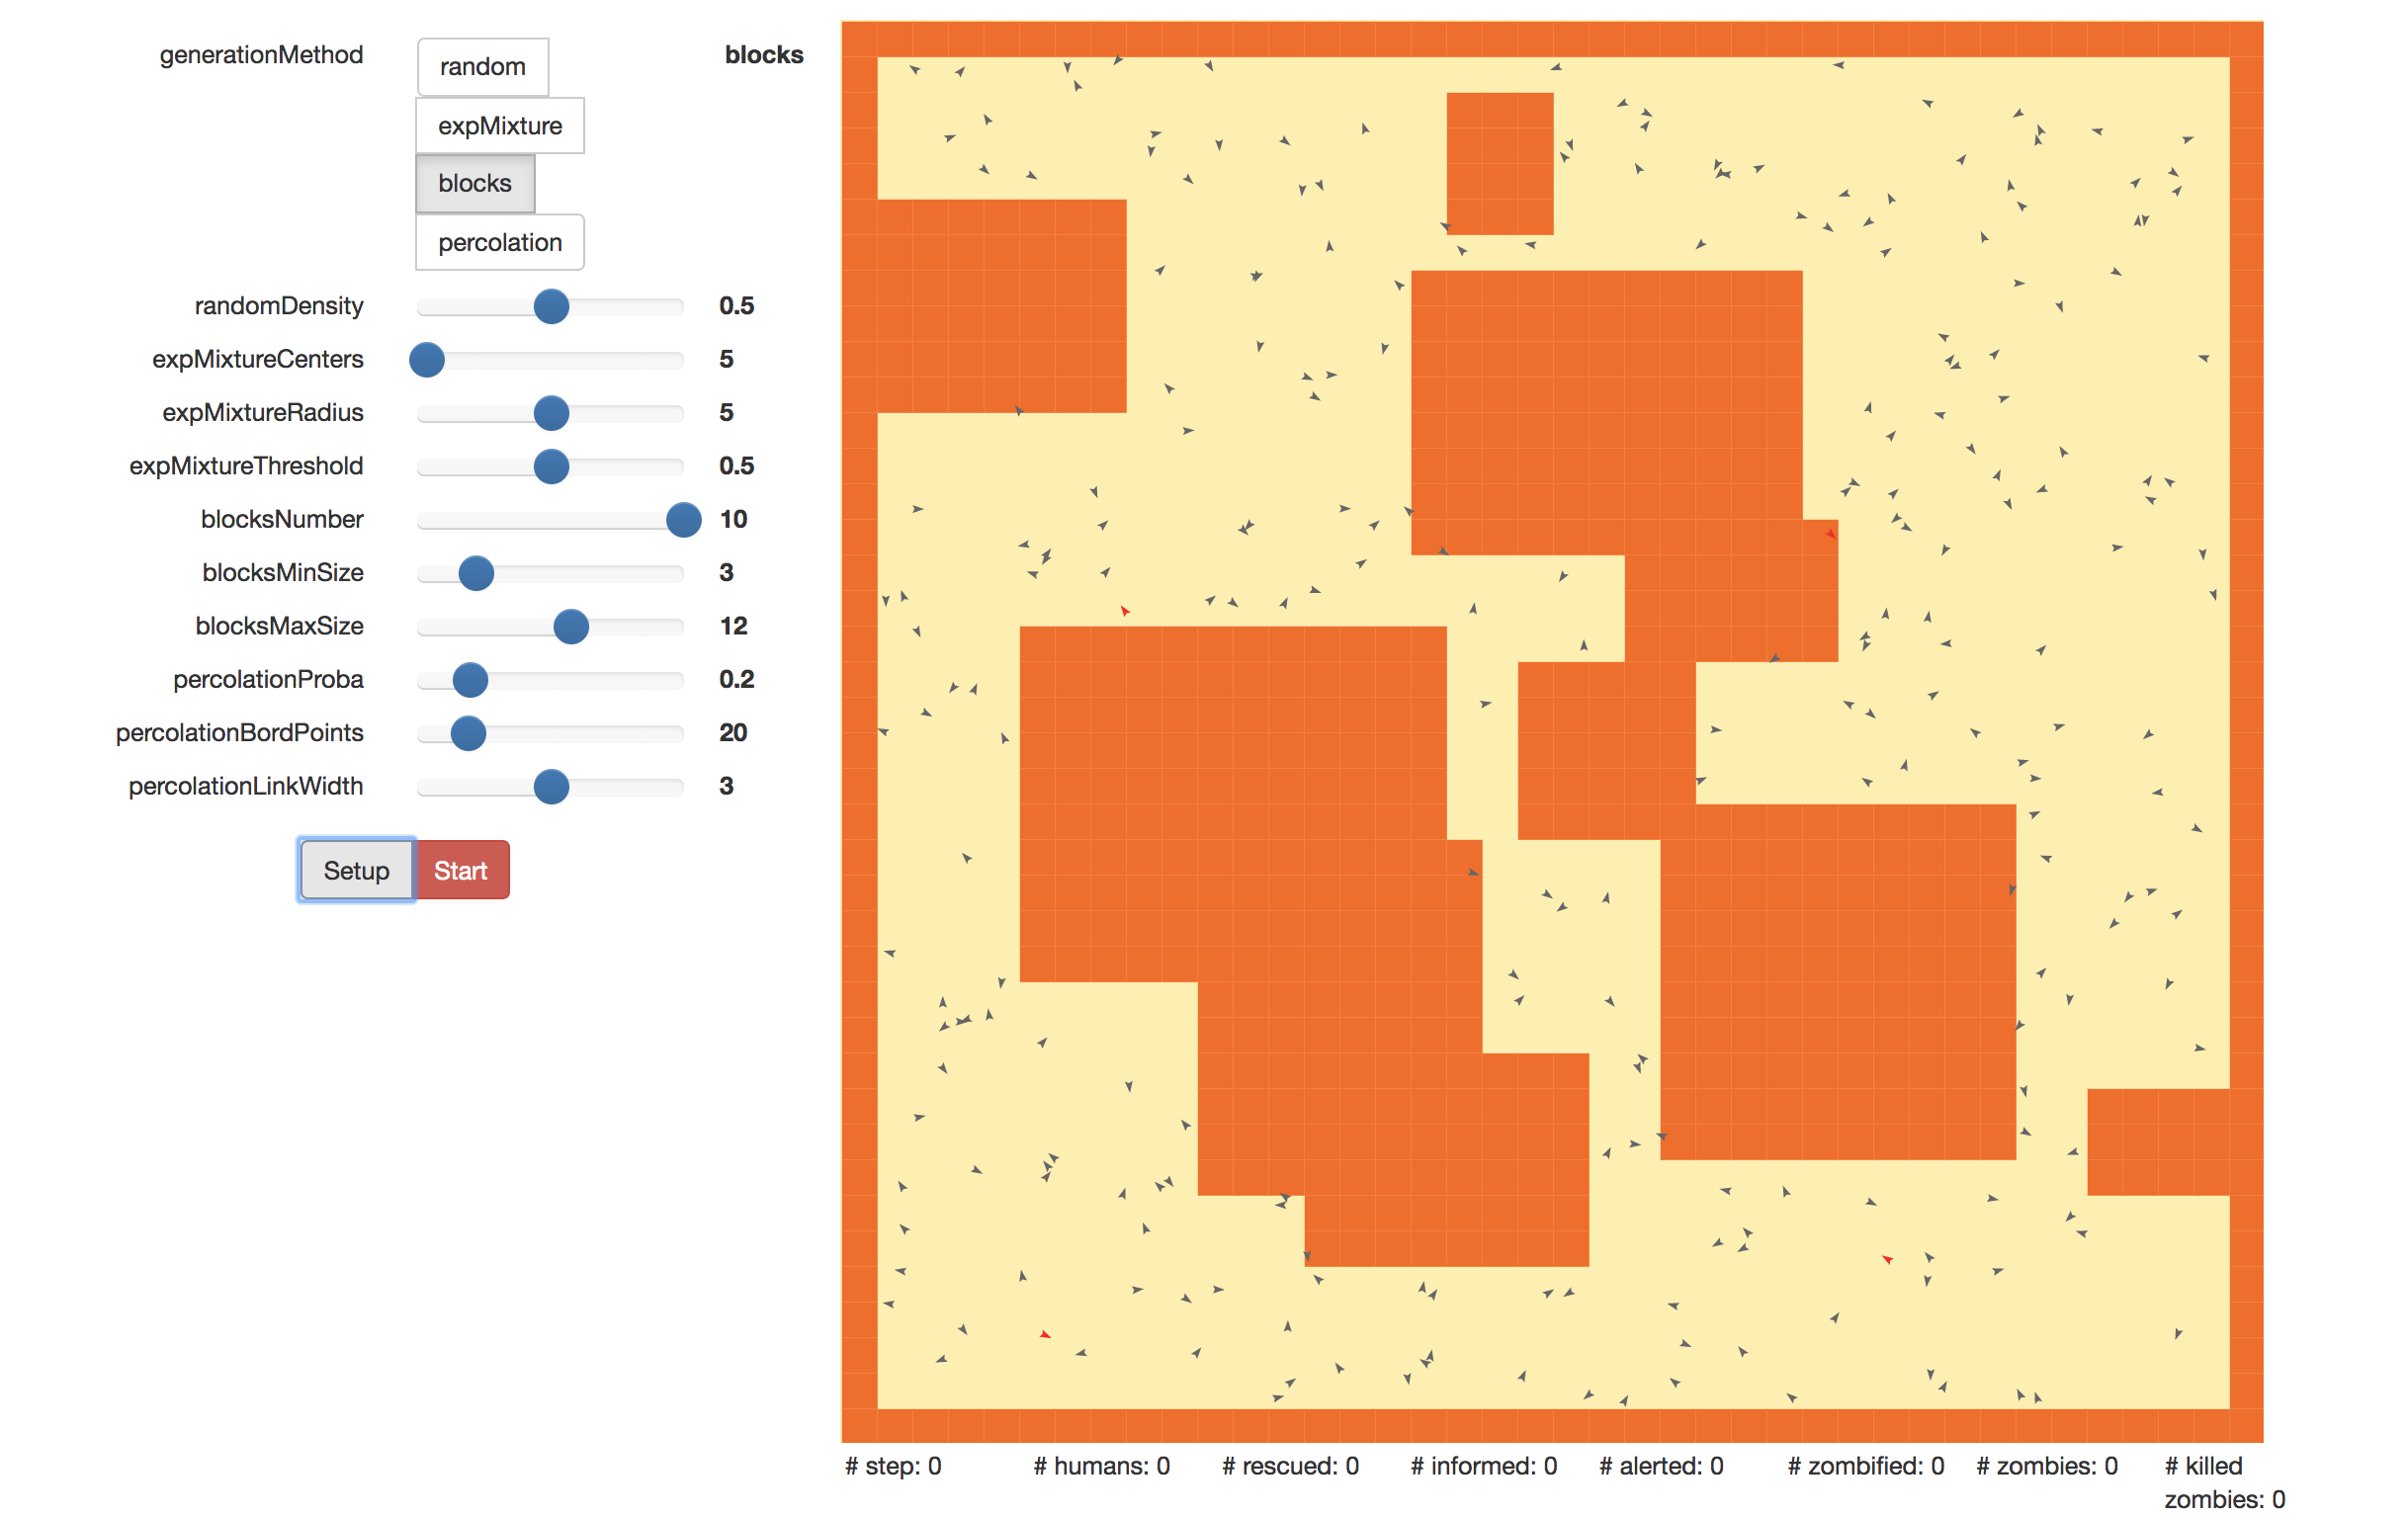
\includegraphics[width=\textwidth]{figures/GUIZOMBIE_spatialsens.png}

}

\sframe{Spatial sensitivity of the Zombie model}{

\textit{Which spatial organization impedes the epidemics?}

\bigskip

\centering

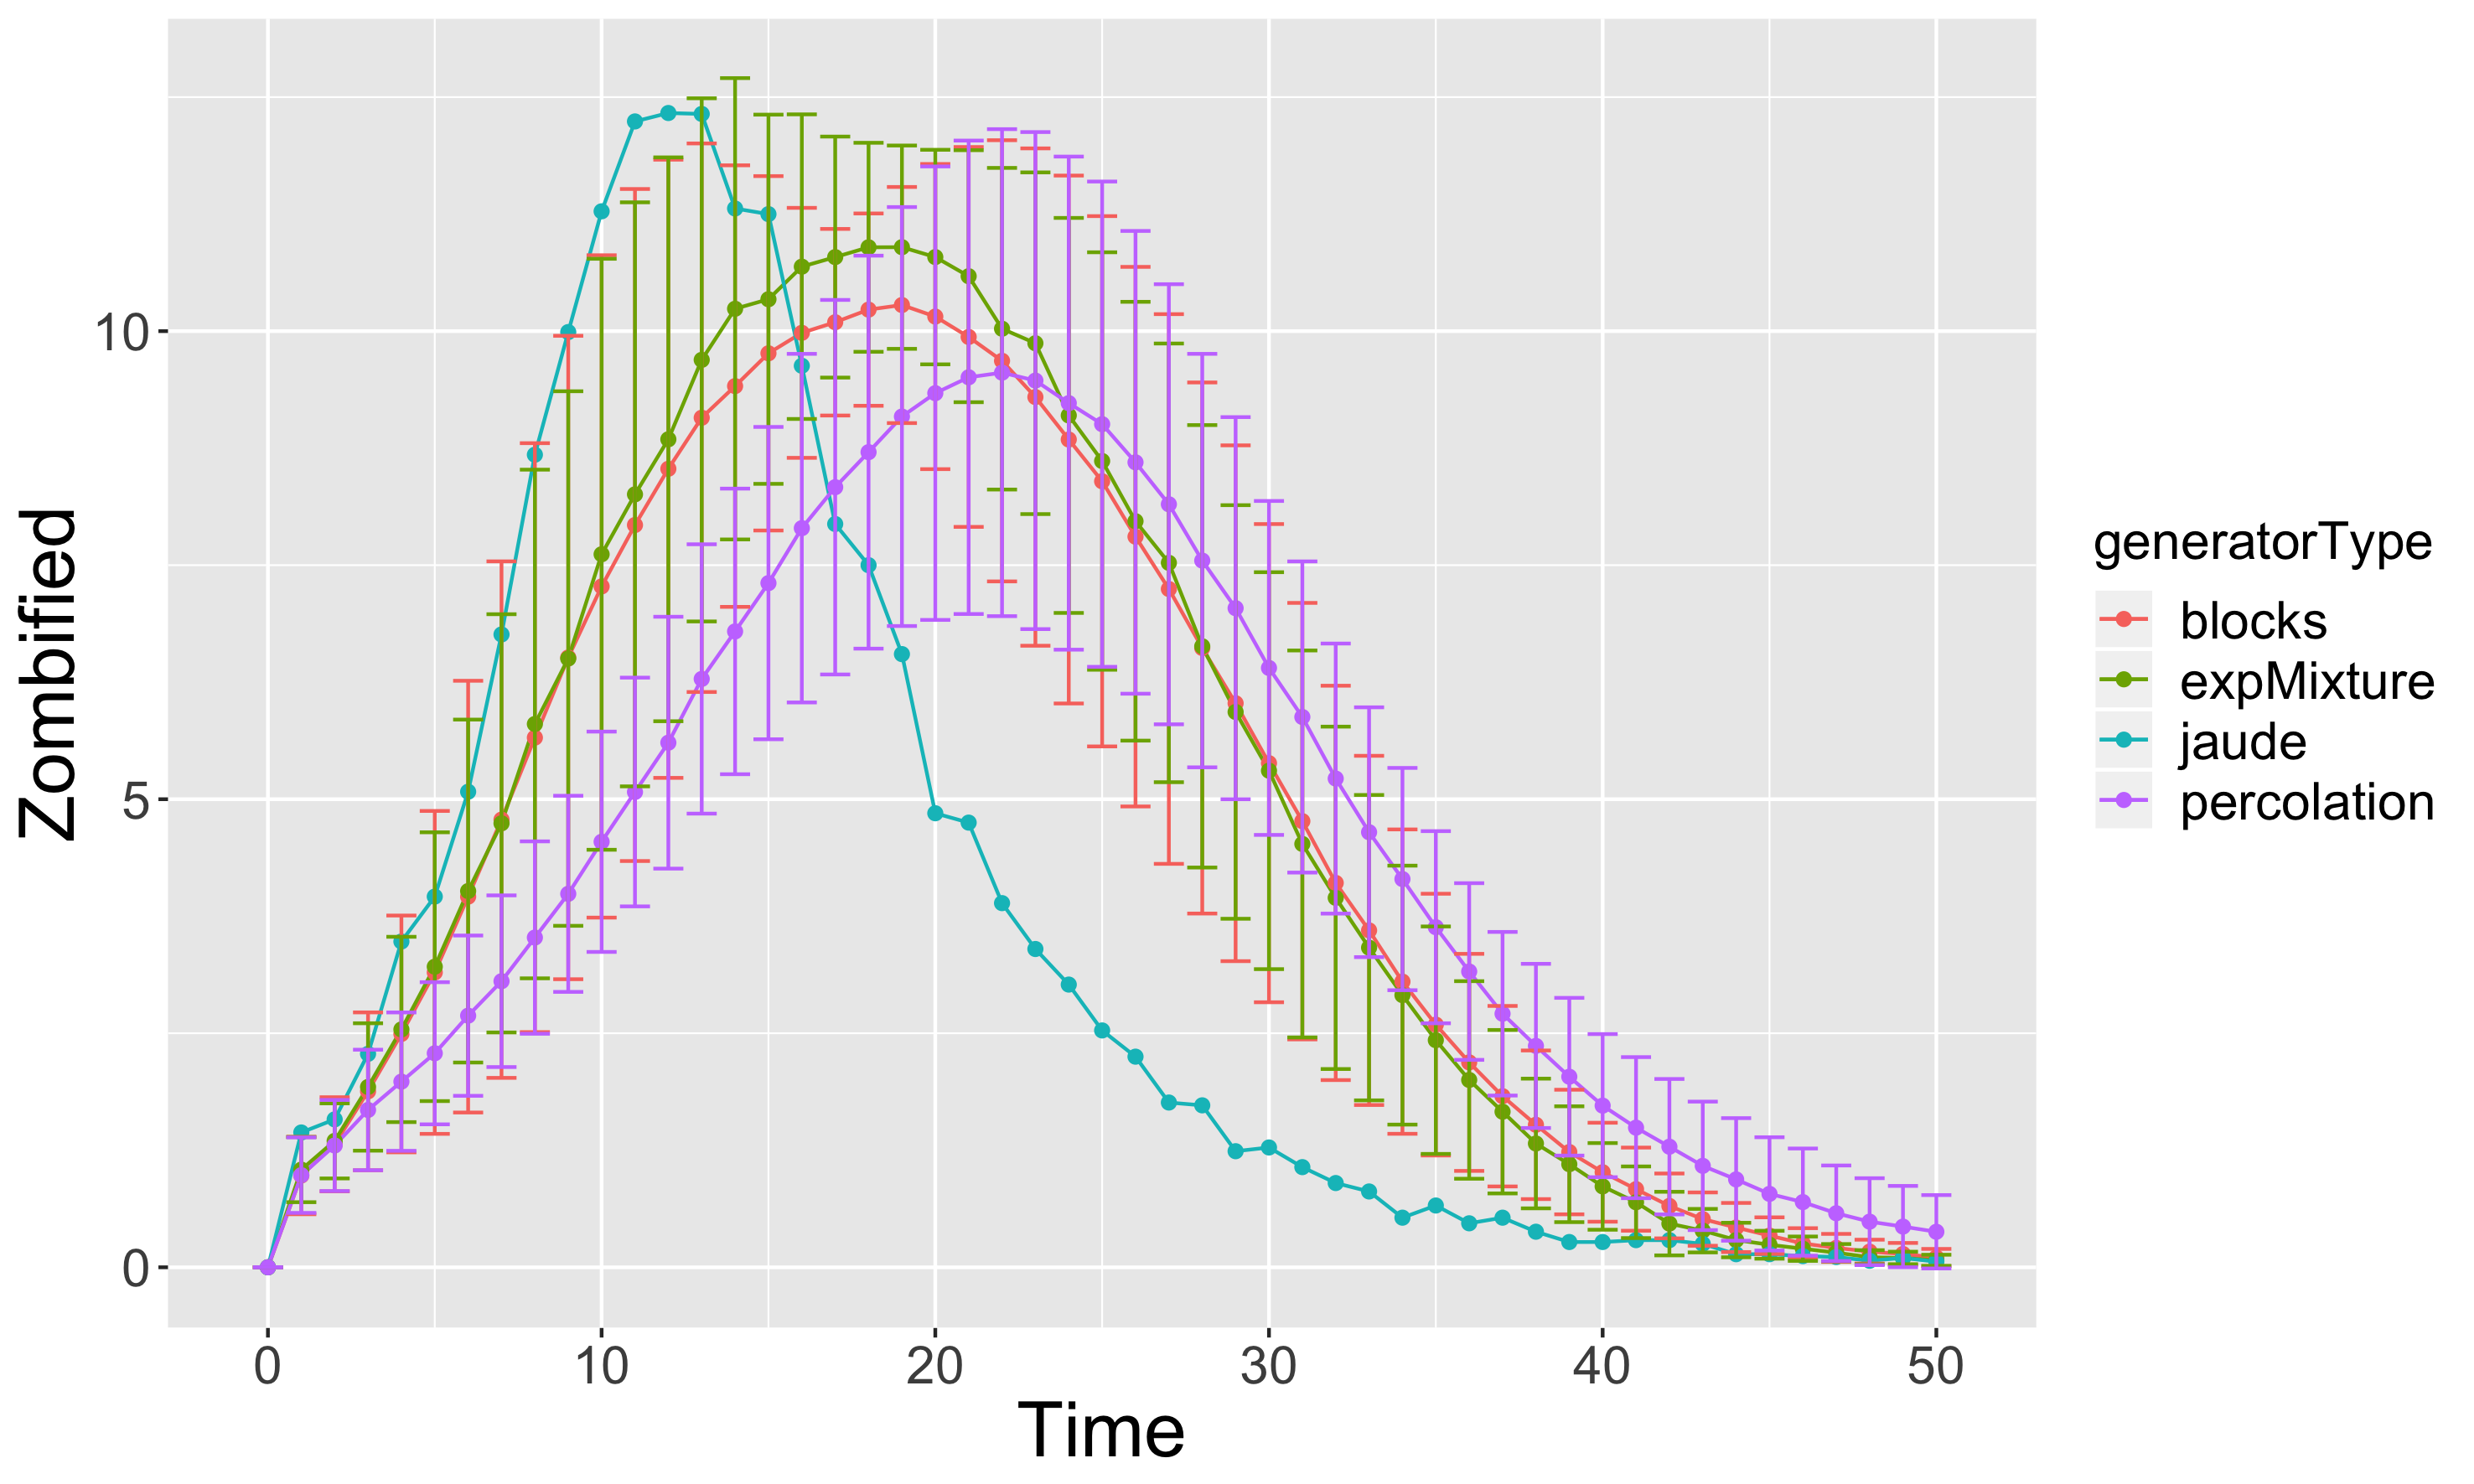
\includegraphics[width=0.58\textwidth]{figures/spatialsens_generators_zombified.png}
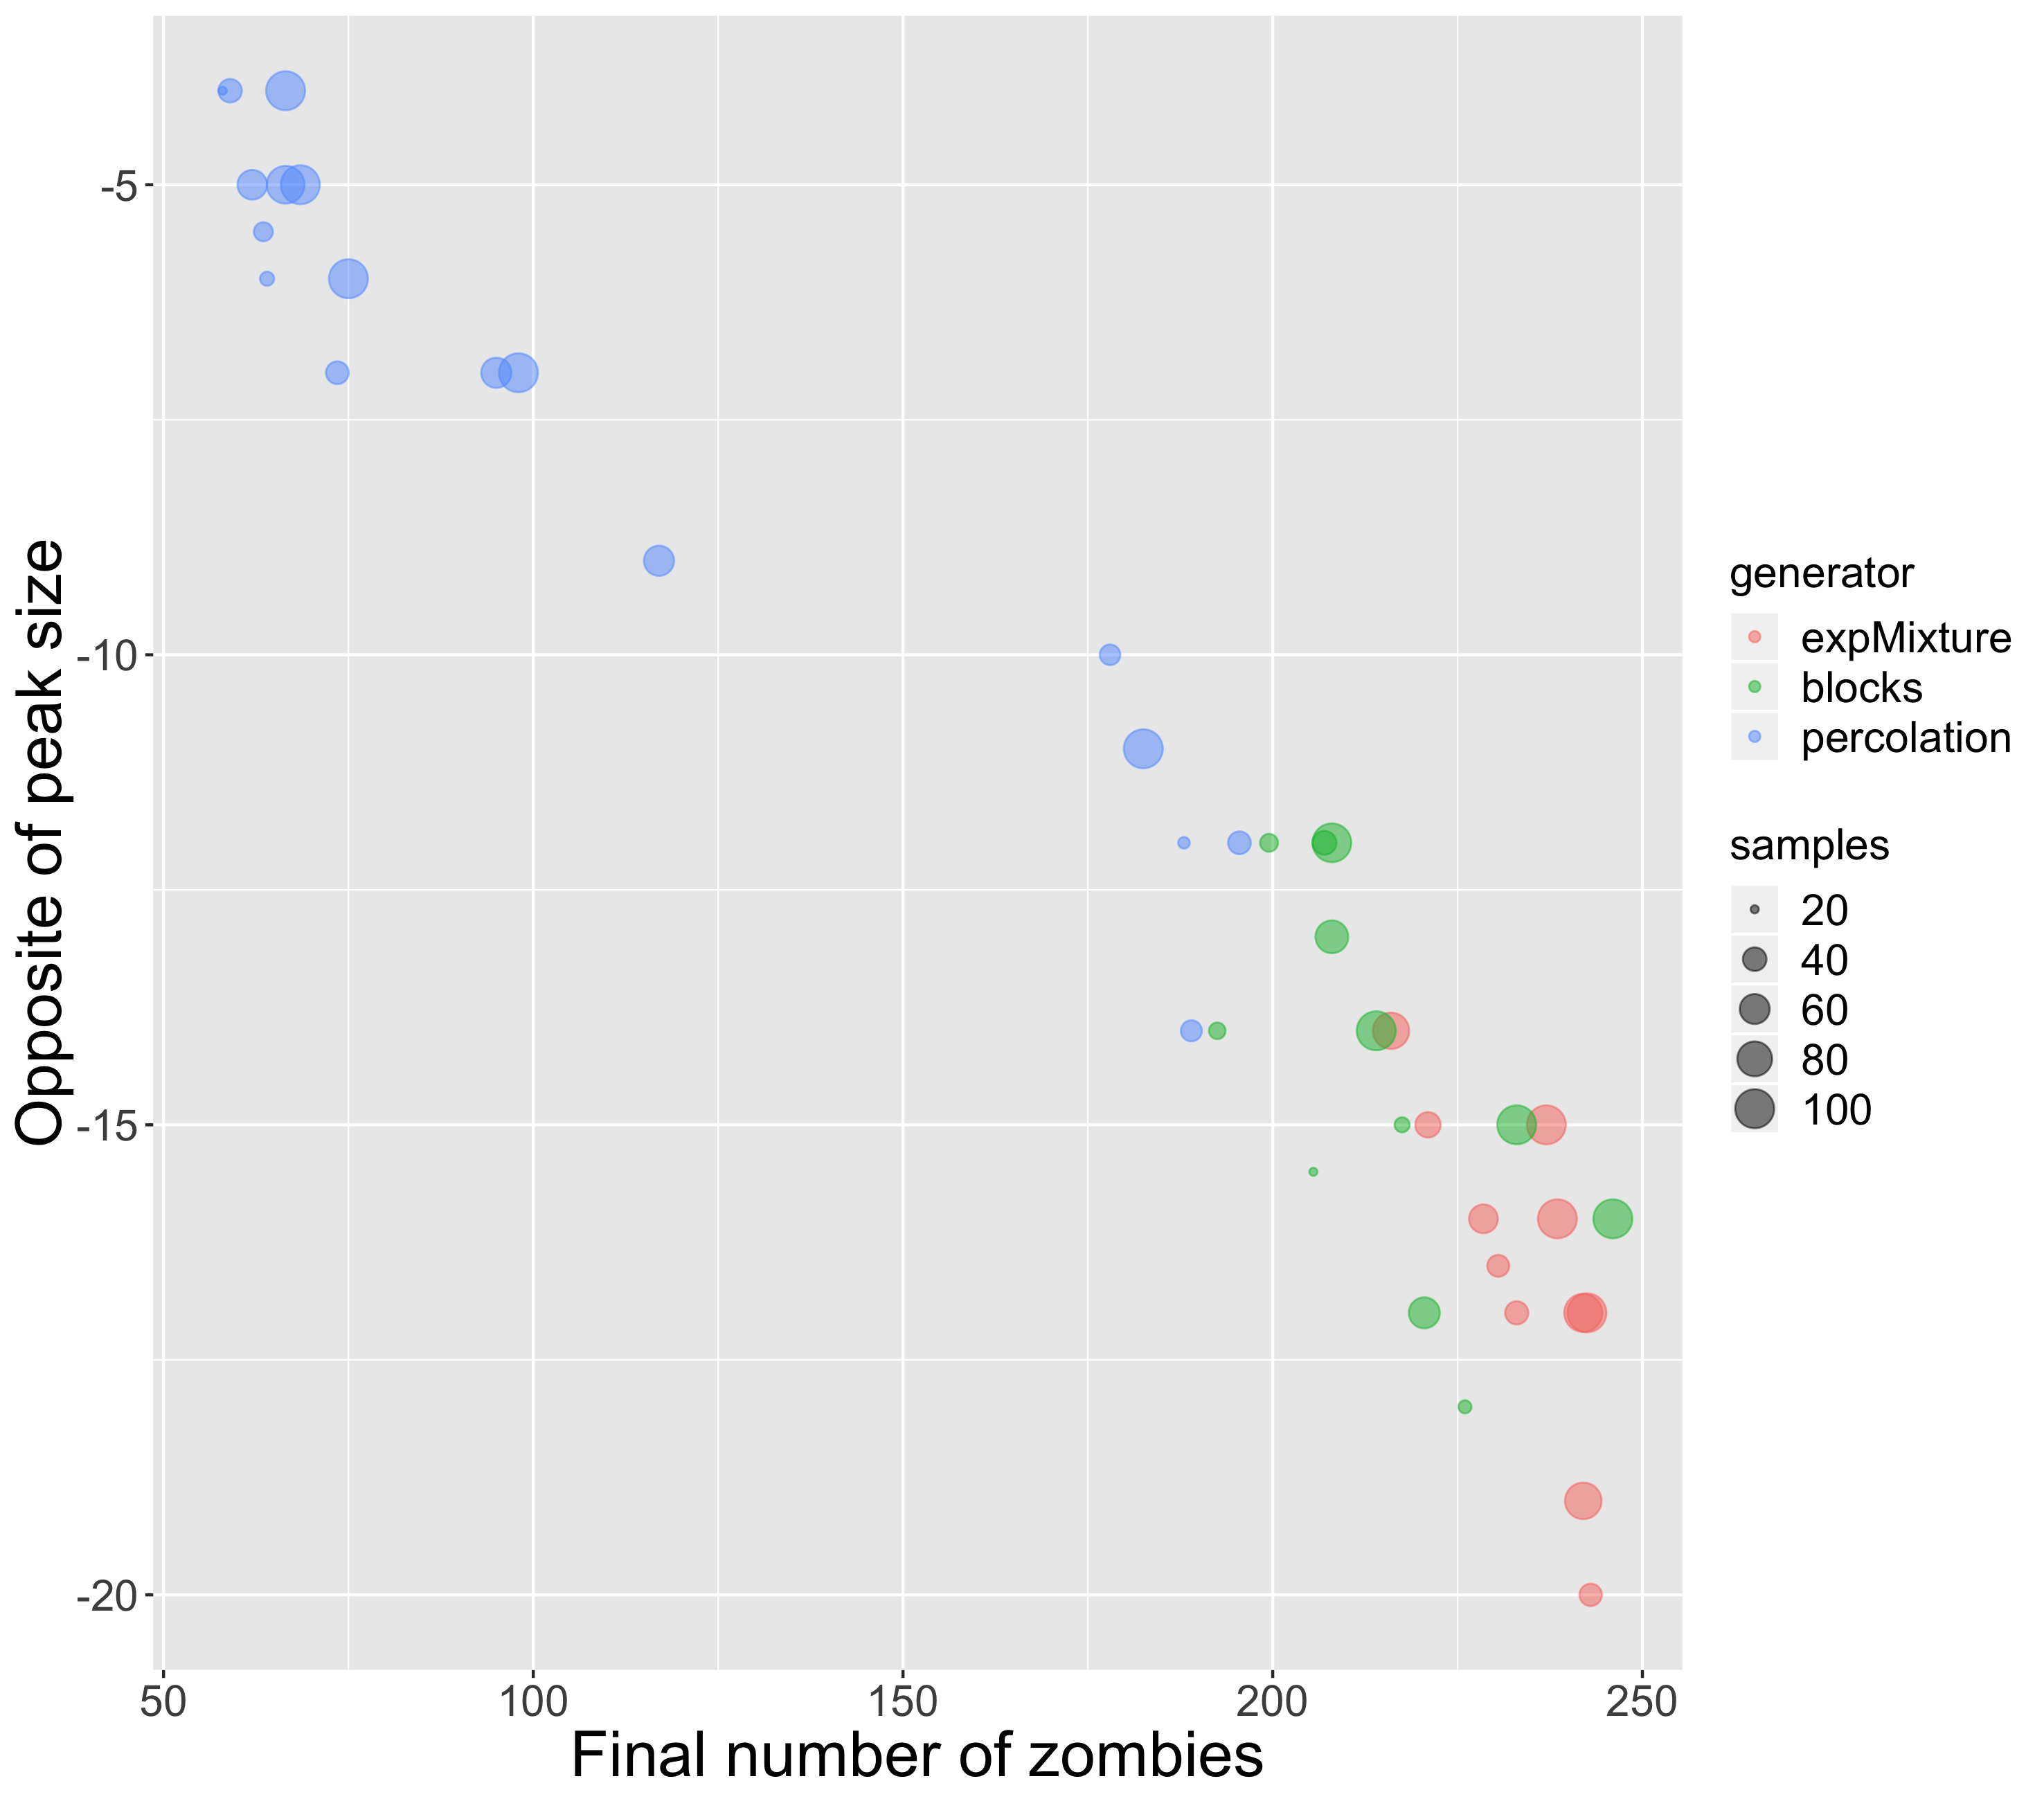
\includegraphics[width=0.4\textwidth]{figures/paretos_20samples.png}


}


\sframe{Specific questions}{

%They are applied on diverse specific submodels, highlighting specific mechanisms of the model, in order to answer associated thematic questions. We also illustrate the comparison with competing model ontologies by calibrating an ODE-based model on data generated by the simulation model.

% - importance of multi-modeling / model comparison / model coupling

\justify
\small

$\rightarrow$ \textit{Study of submodels to foster diverse questions and approaches: cooperation between humans, army intervention, red cross and vaccination}


\medskip


$\rightarrow$ \textit{Comparison of the ABM with alternative formalisms}

\medskip

\centering

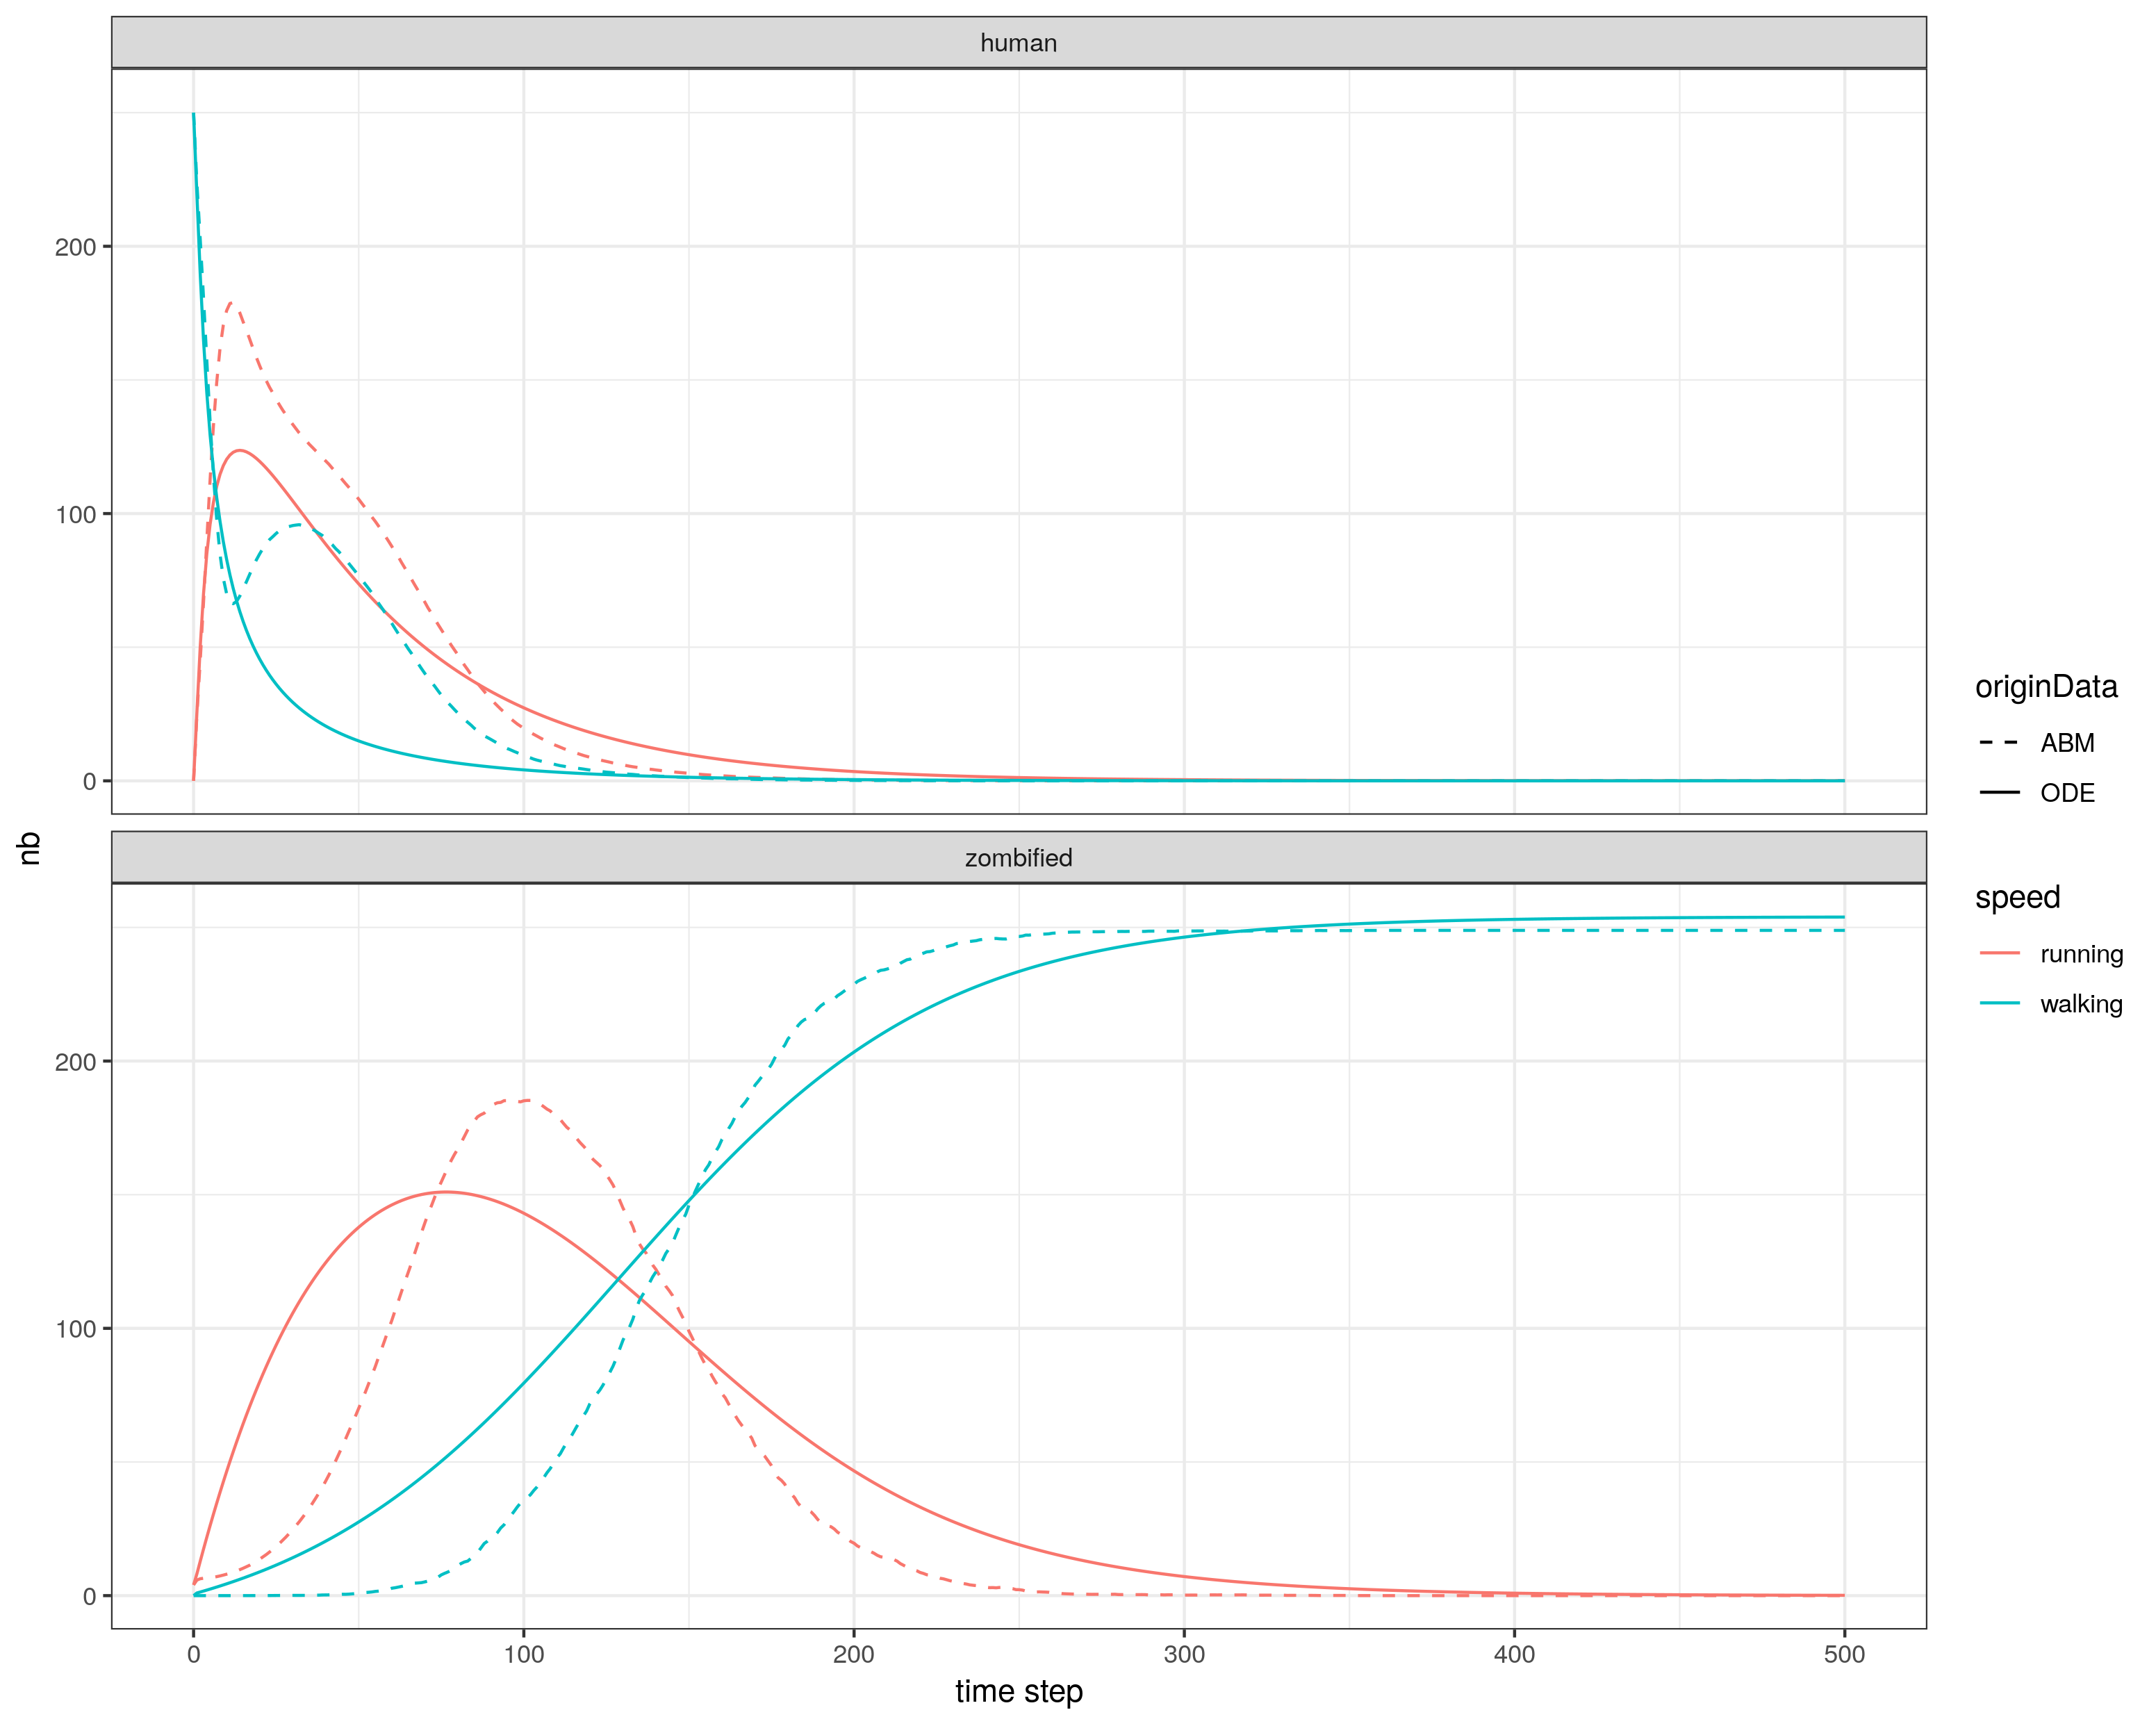
\includegraphics[width=0.7\textwidth]{figures/parcimony_dynamics_2.png}

\small
\textit{Regimes of ABM compared to ODE patterns}

}


\sframe{Synthesis: challenge}{

%We finally synthesize lessons learned in the final challenge part of the school, consisting of the autonomous exploration of a new model instance by participants, including defining a thematic question and applying appropriate validation methods.

% - openness is crucial (define their own questions)
% - no direction taken had been previously thought
% - not that much need to interact with model code (a few did)

A \textbf{student challenge} for autonomous practice 

$\rightarrow$ they define a fresh thematic question 

$\rightarrow$ they define the adequate design of experiments, especially methods and measures.

$\rightarrow$ possibly model code modification

\bigskip

\centering
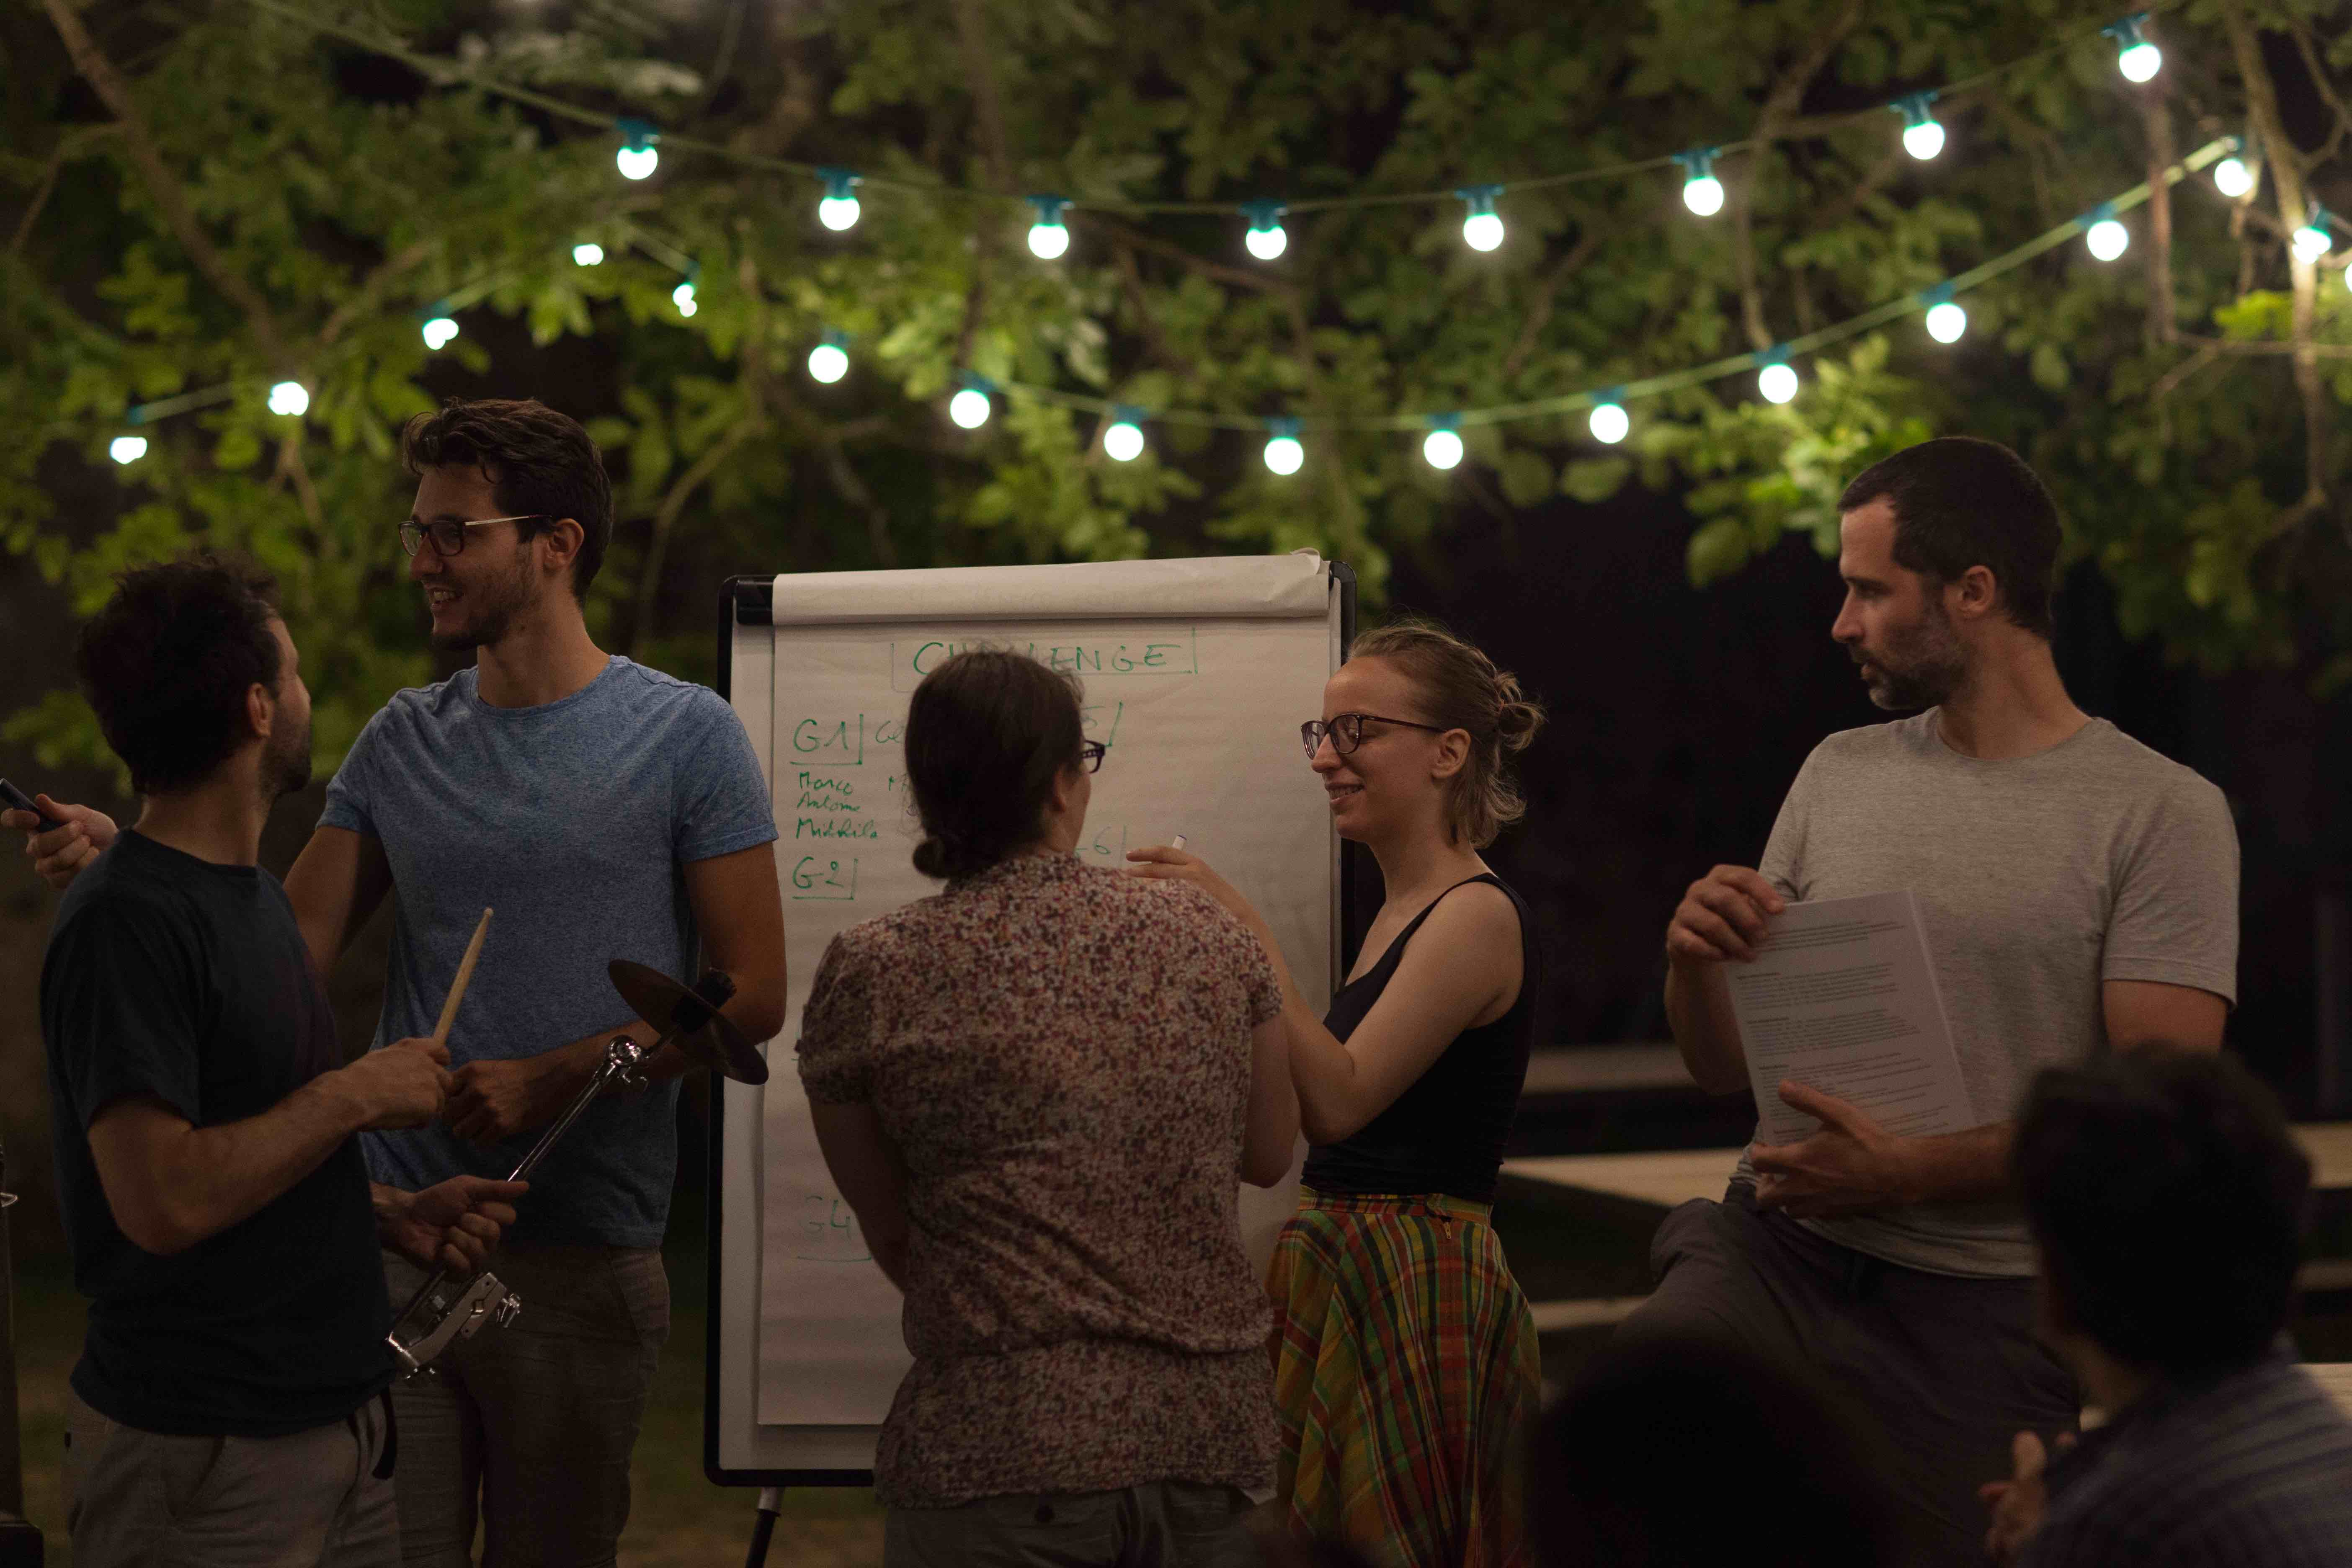
\includegraphics[width=0.7\textwidth]{figures/exmodelo-challenge_IMG_3876_LR.jpg}


}


\sframe{Challenge results}{

\textit{Each group came with unforeseen questions and ideas; not much advanced methods where however used}

\medskip

\centering

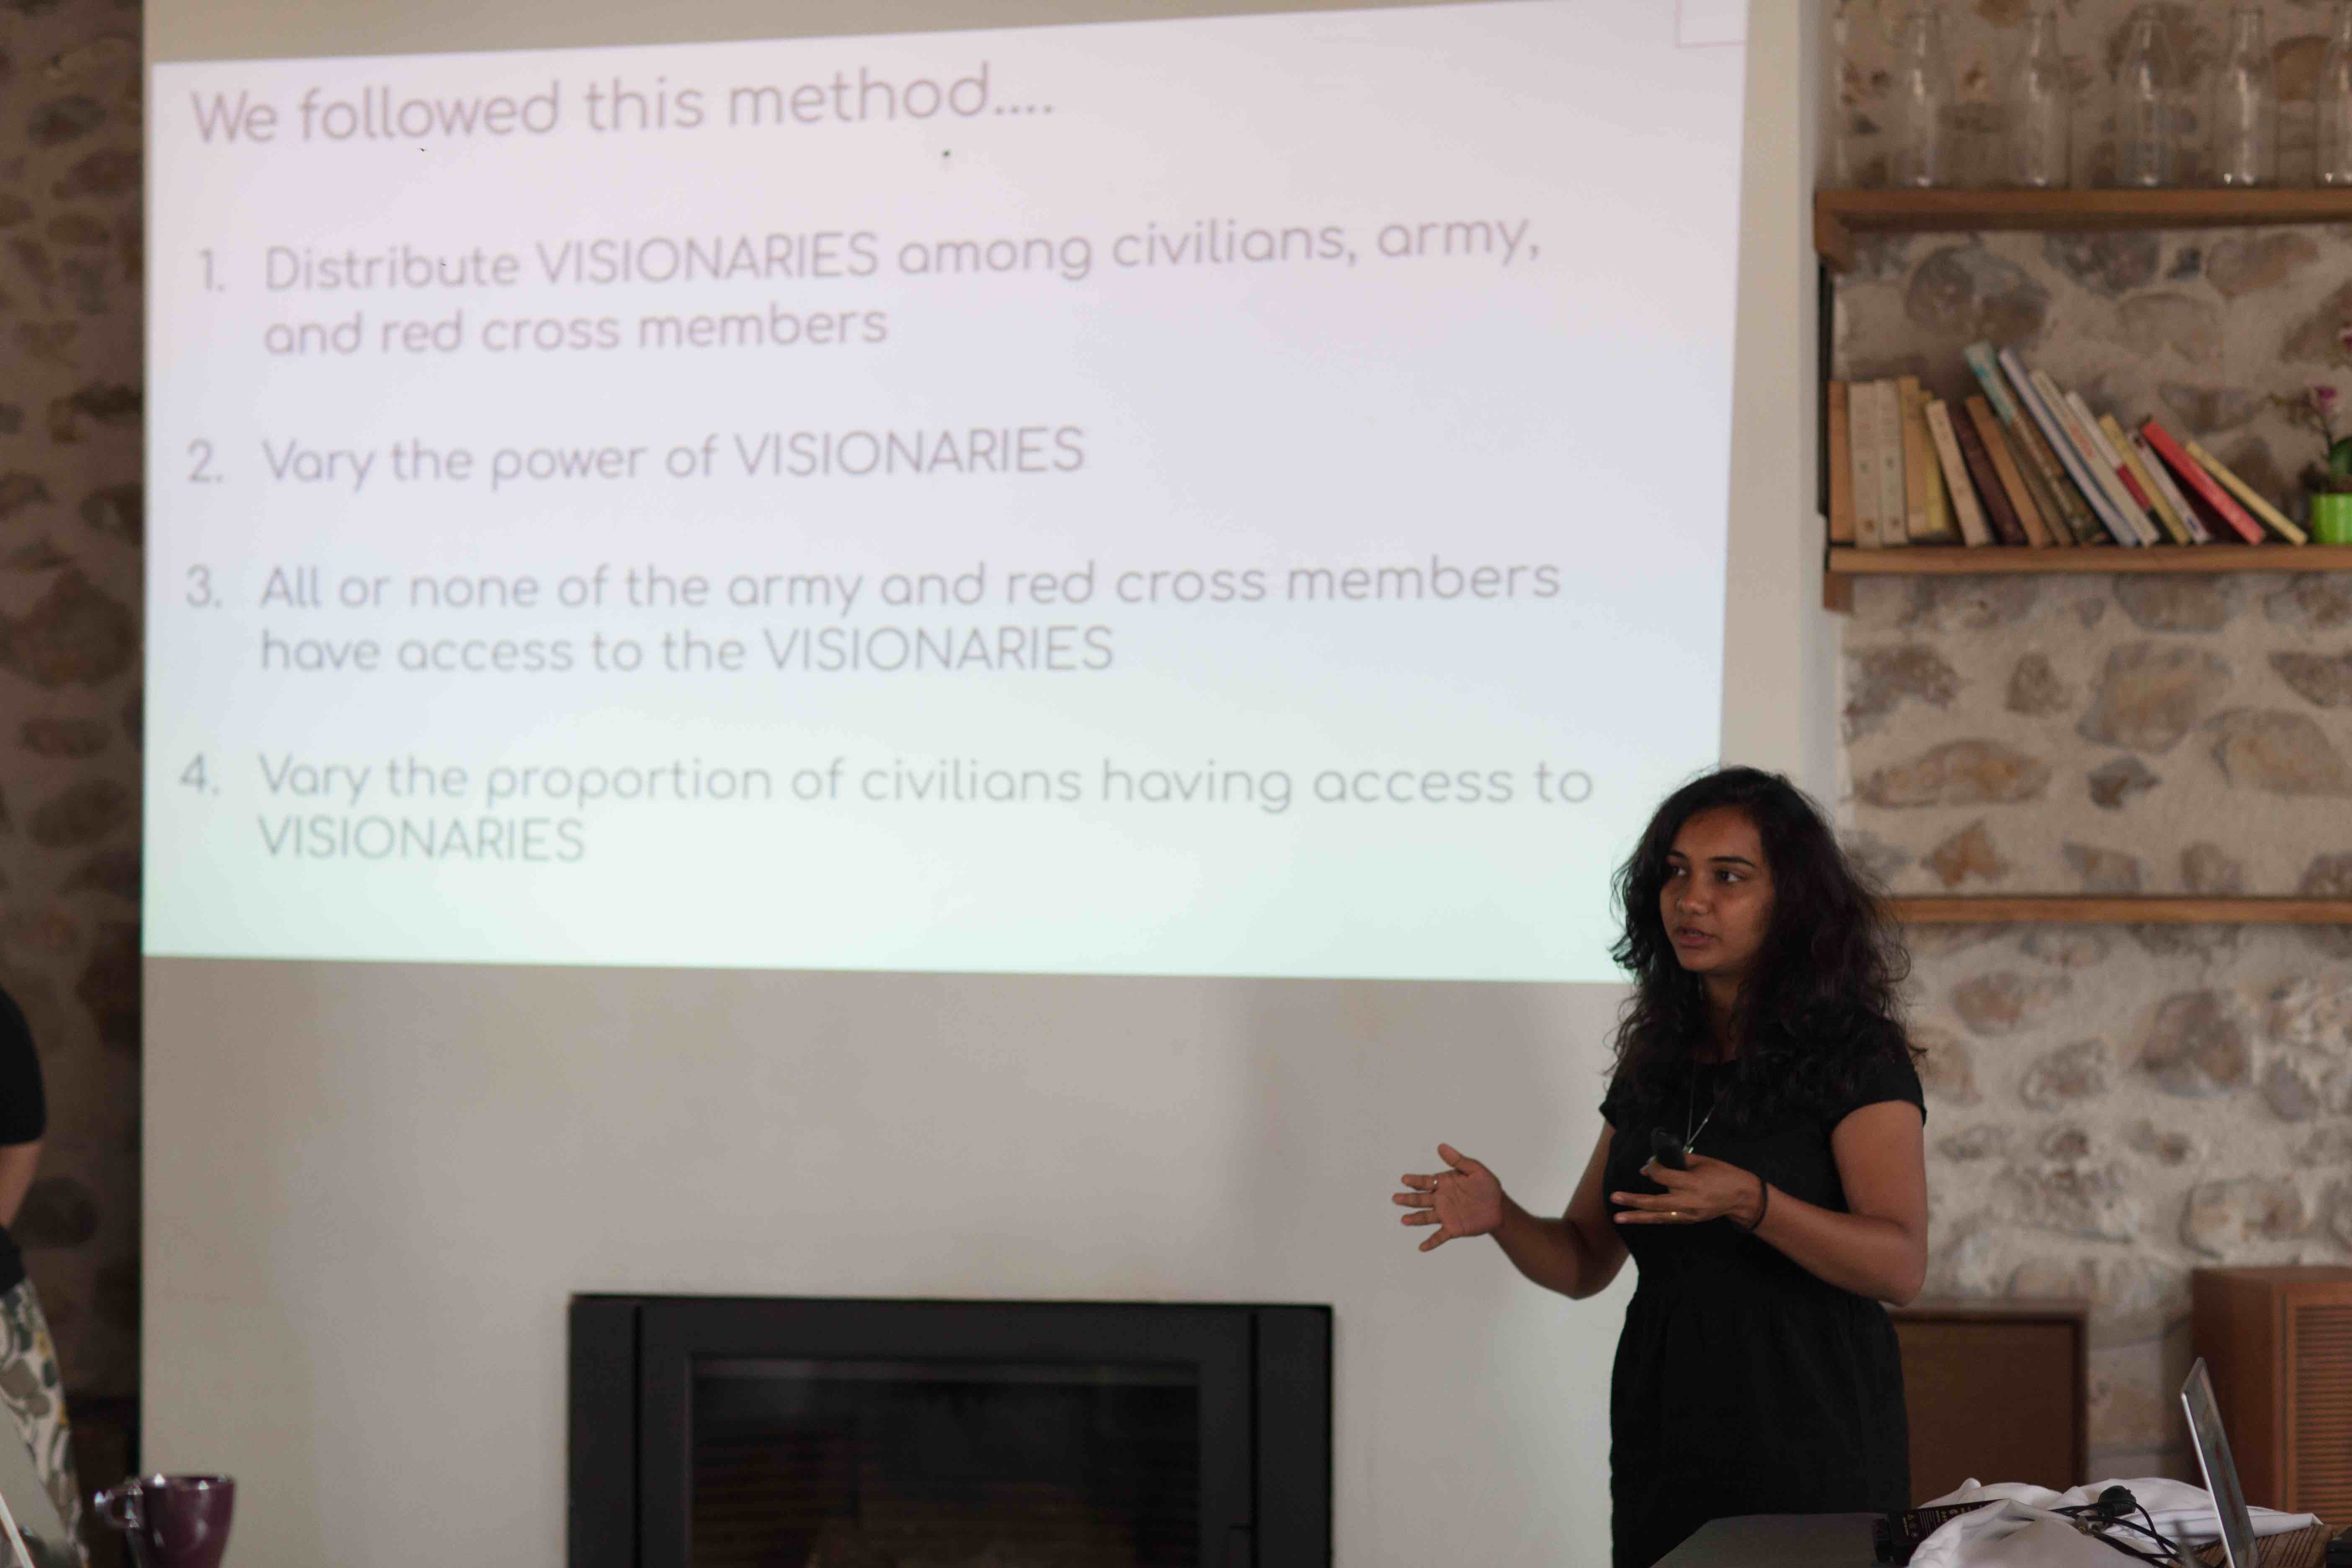
\includegraphics[width=0.45\textwidth]{figures/exmodelo-vision_IMG_4101_LR.jpg}\hspace{0.1cm}
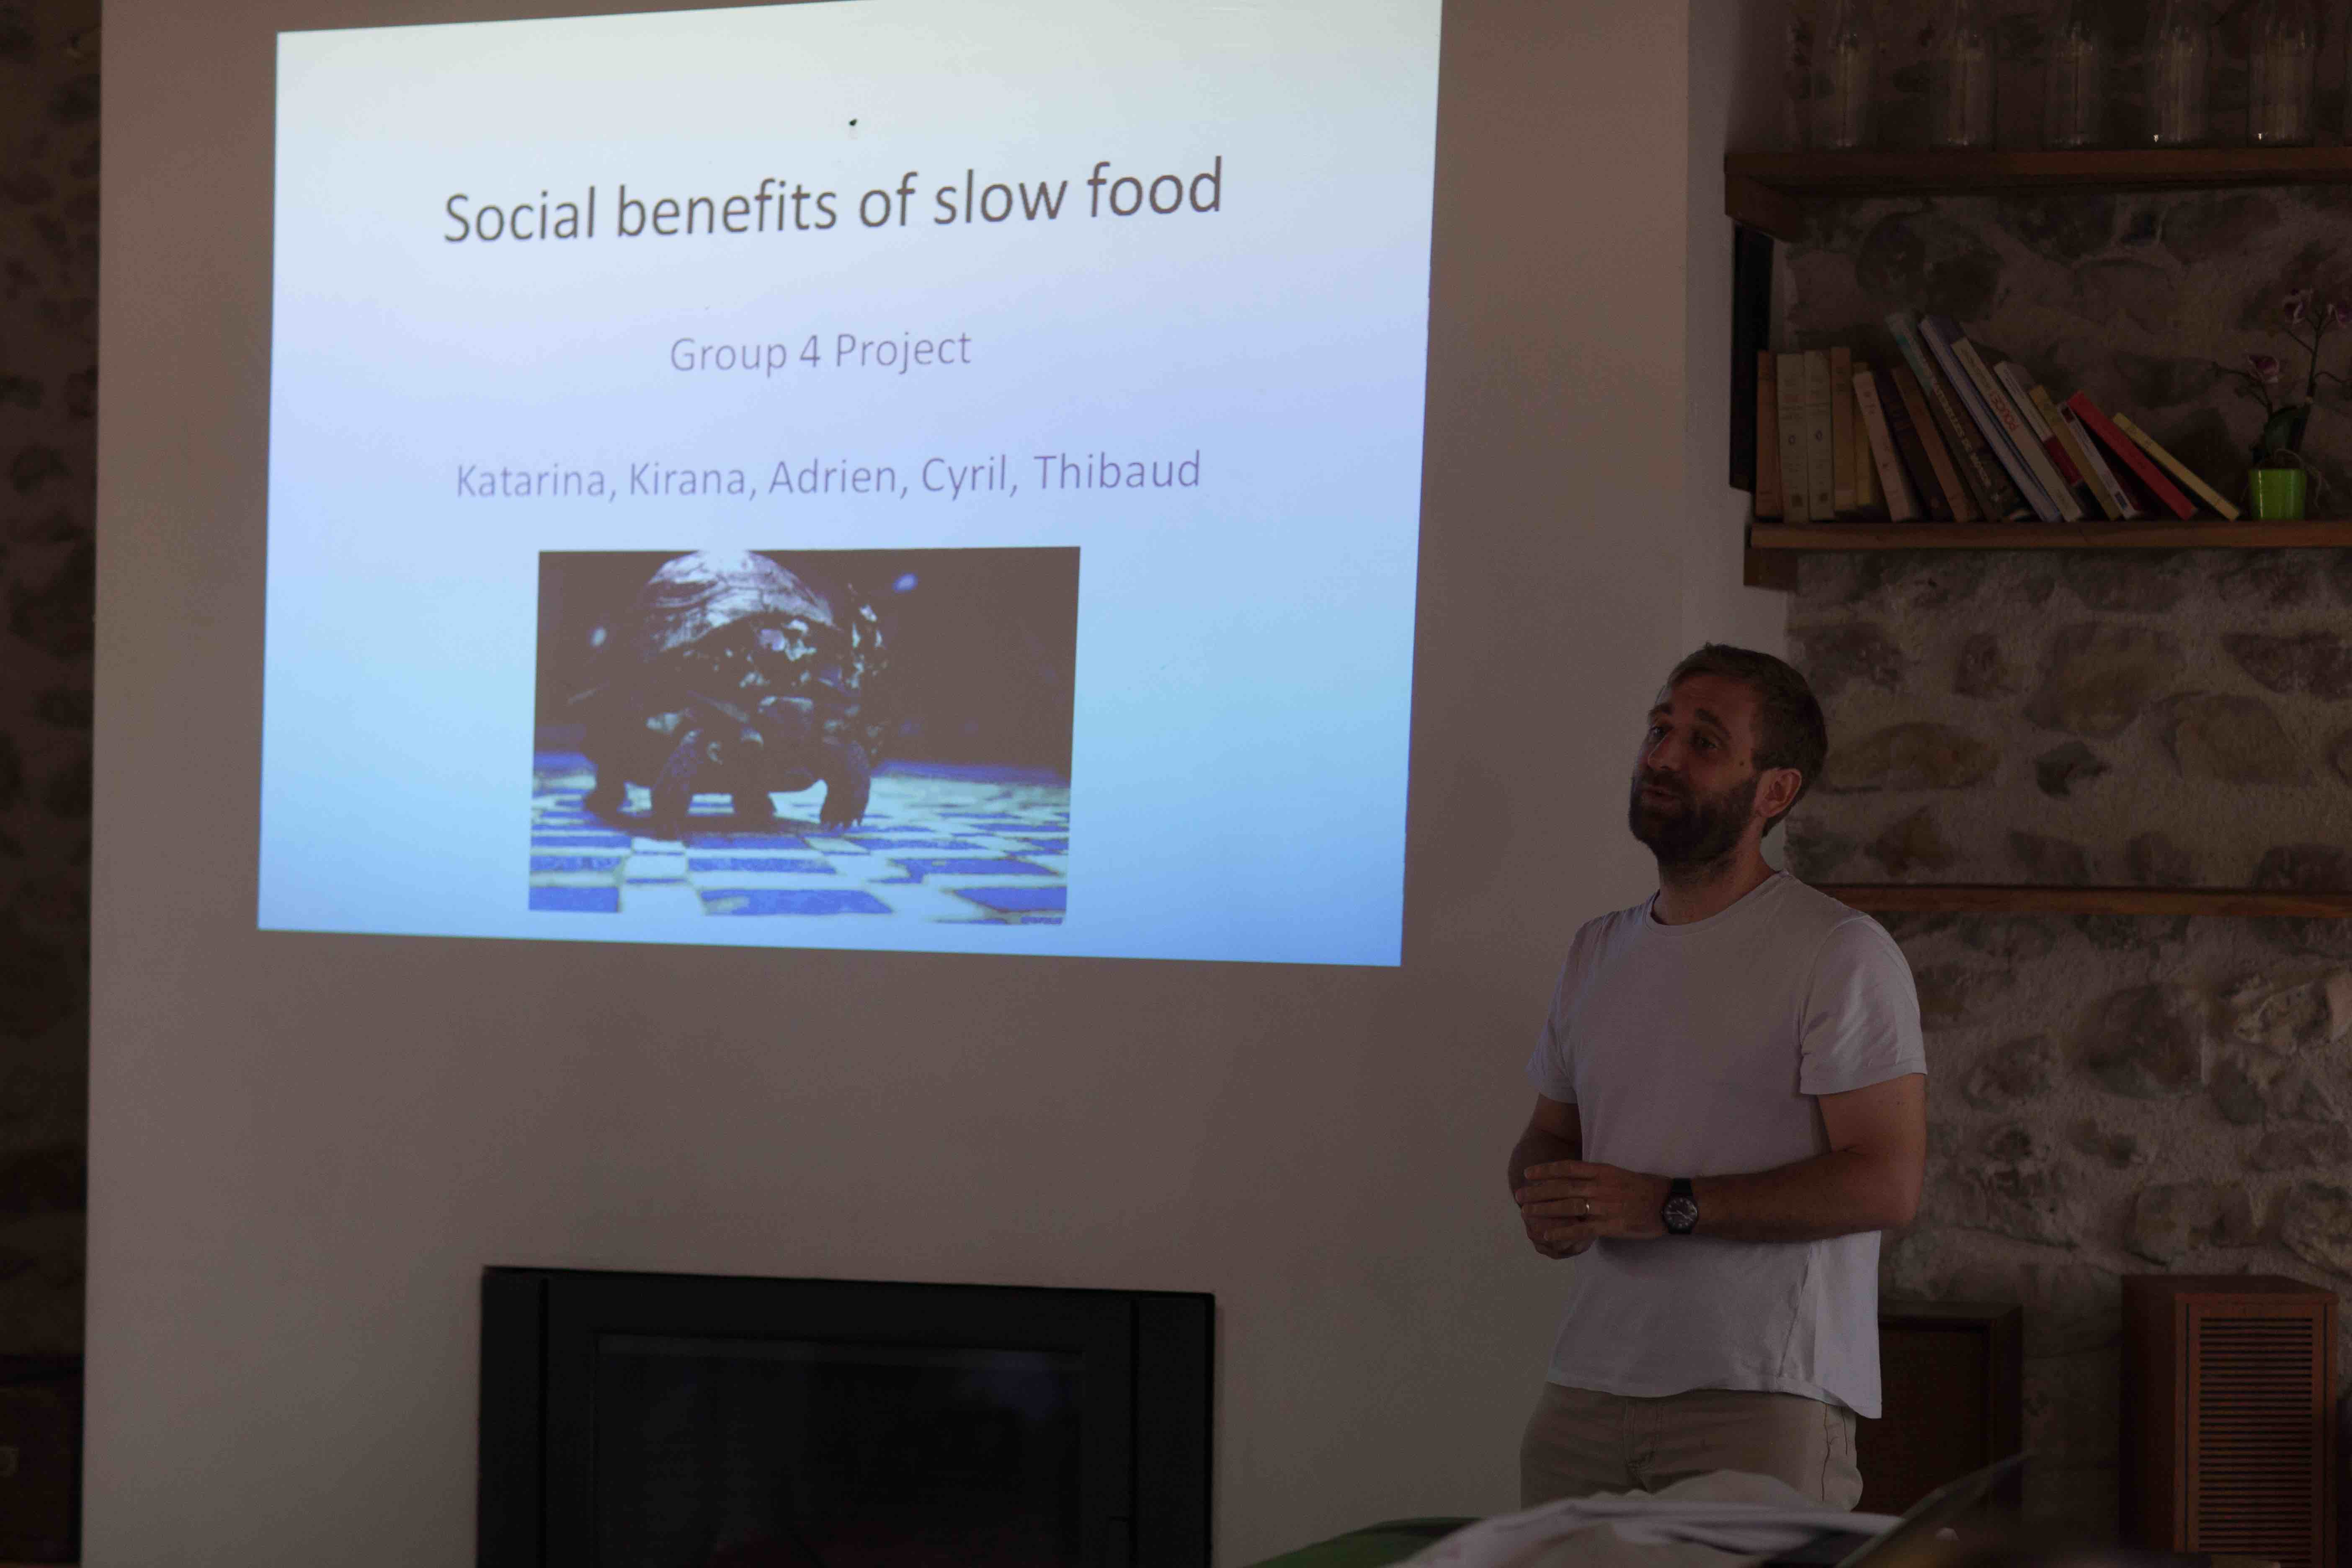
\includegraphics[width=0.45\textwidth]{figures/exmodelo-slowfood_IMG_4172_LR.jpg}\\\vspace{0.1cm}
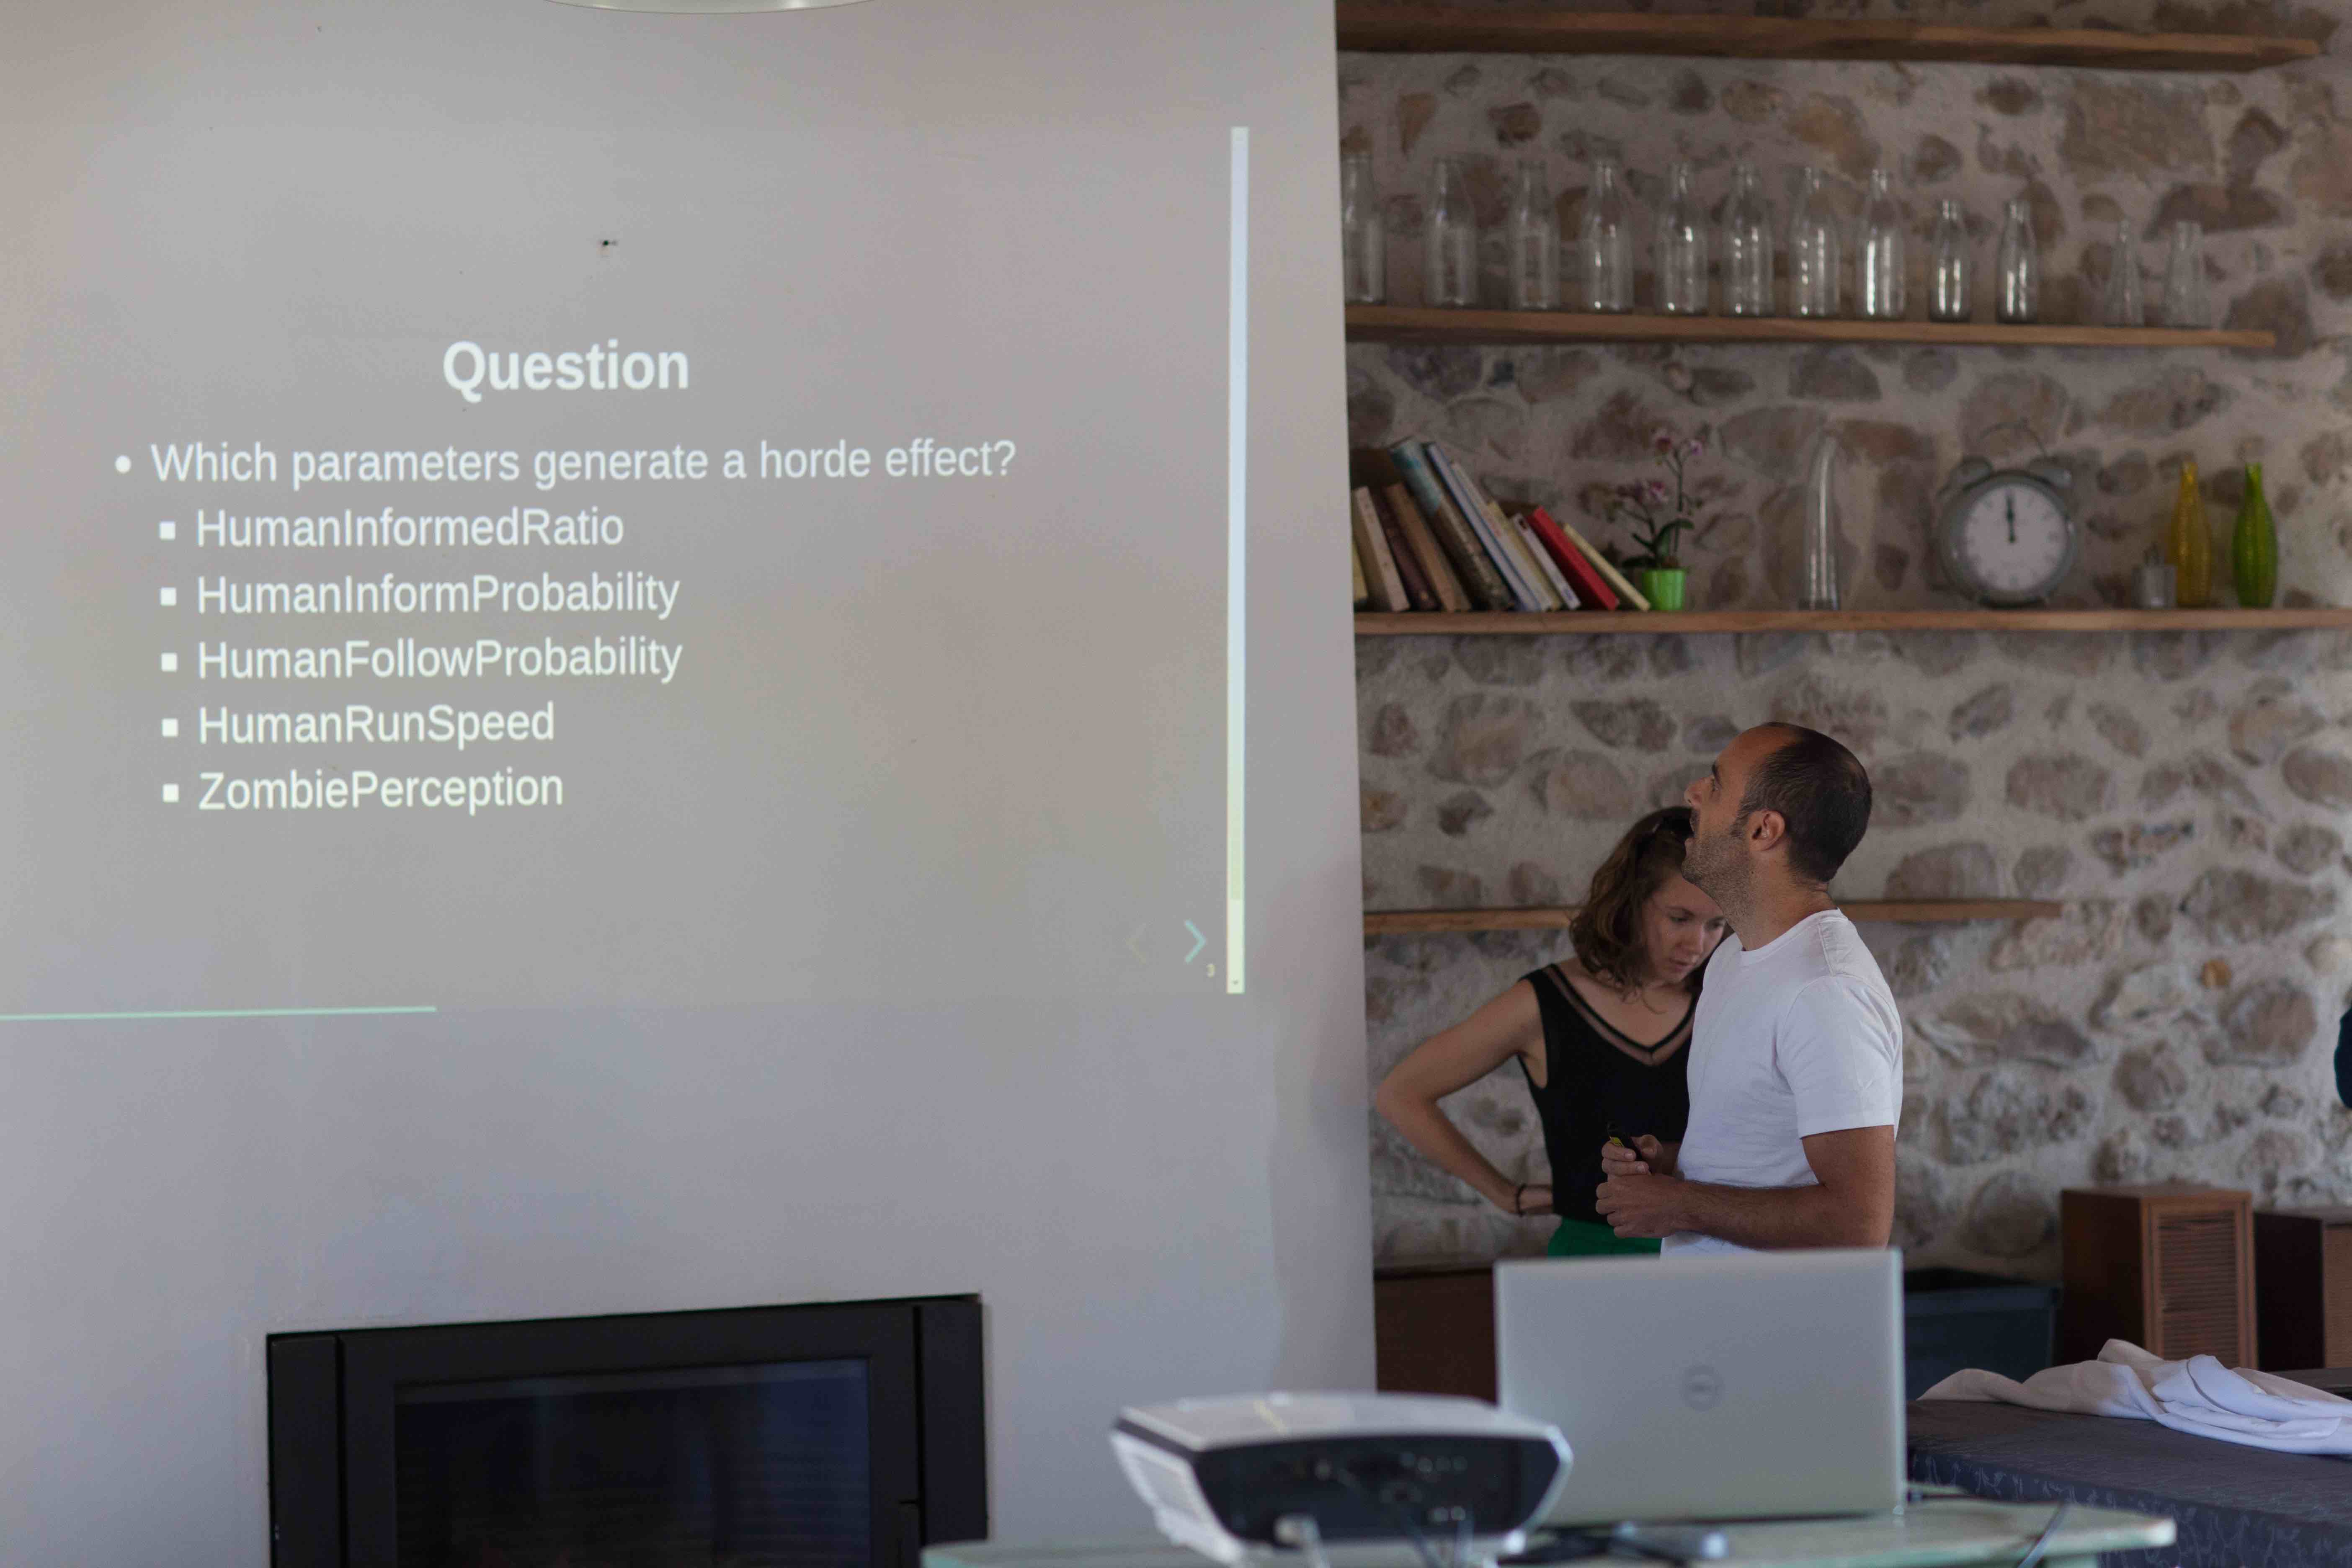
\includegraphics[width=0.45\textwidth]{figures/exmodelo-horde_IMG_4208_LR.jpg}\hspace{0.1cm}
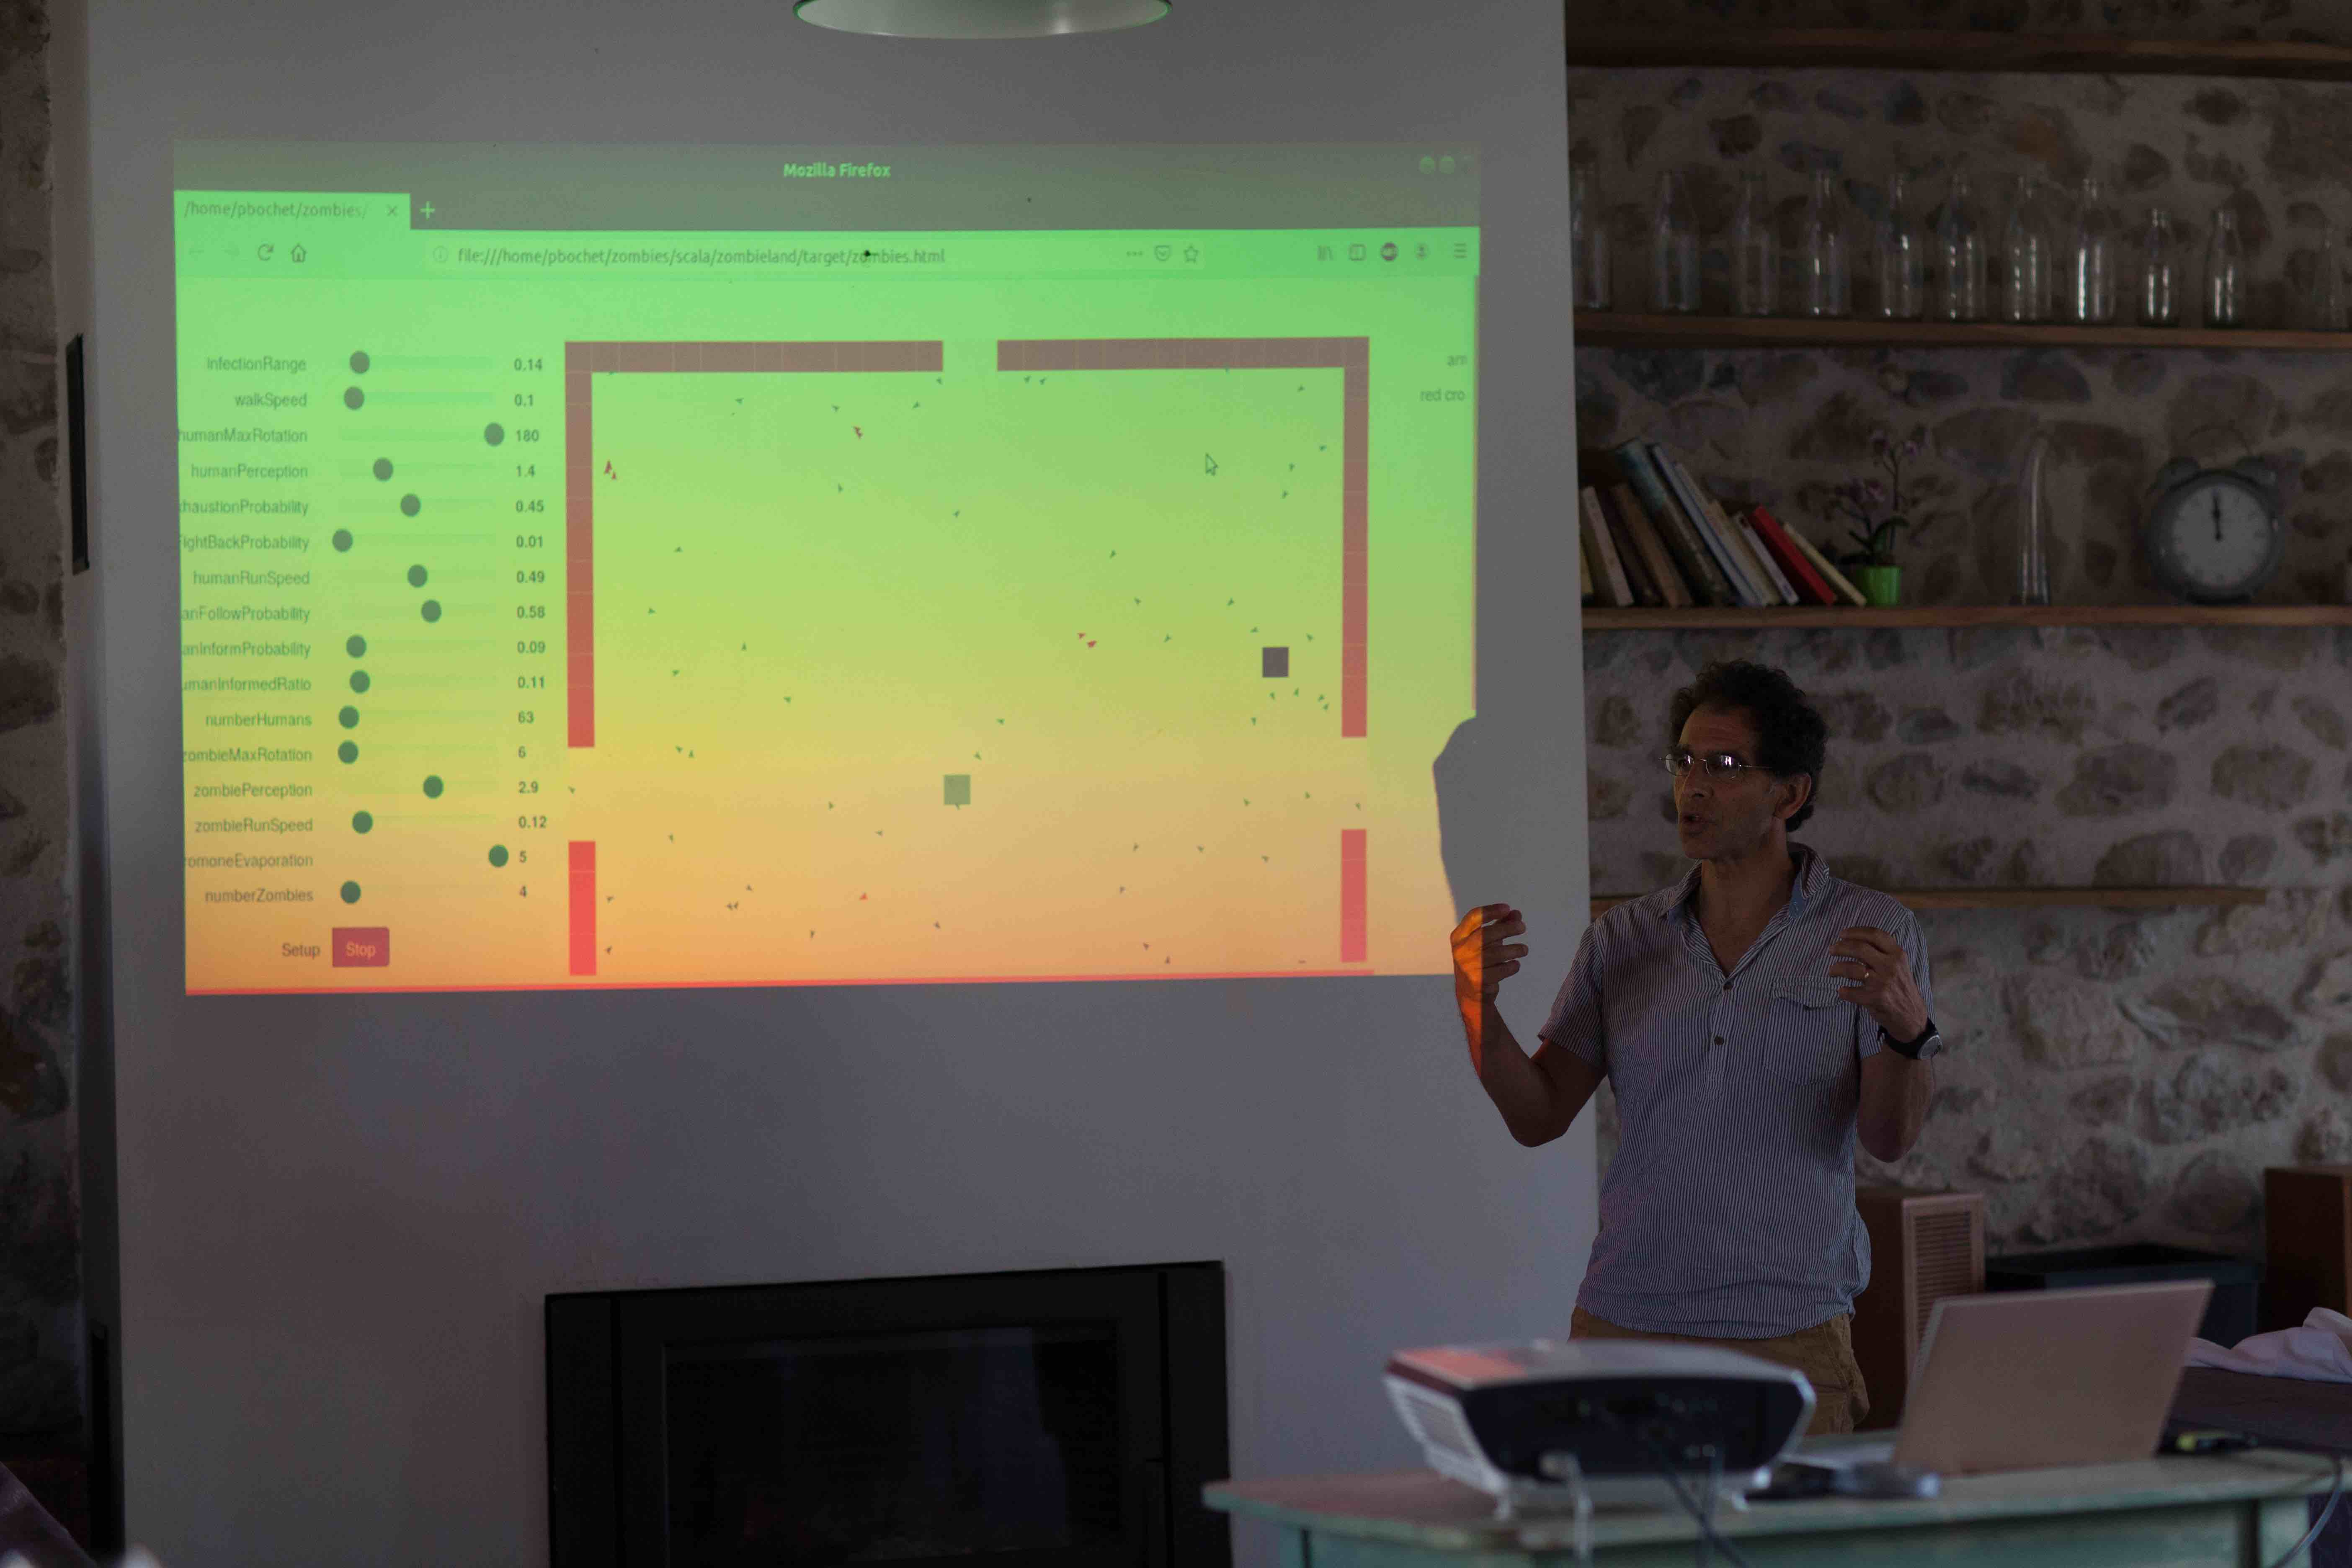
\includegraphics[width=0.45\textwidth]{figures/exmodelo-stationary_IMG_4157_LR.jpg}



}



\sframe{Discussion : Pedagogical Implementation}{

%This experiment both introduces a broad overview of new geosimulation model methods, and suggests ways to disseminate these into the modeling communities through similar pedagogical implementations.

% - importance of the progressive introduction of methods / a full set / mindset . (different from reading a specific hard technical paper about the super new method)


Goals :
\begin{itemize}
    \item Balancing theory and practice 
    \item Flattening disciplinary heterogeneity 
    \item Focusing on model analysis methods instead of platform/framework  
\end{itemize}
\bigskip
Expected benefits :
\begin{itemize}
    \item Methods and approach dissemination
    \item OpenMOLE visibility improvement %à voir si on veut promouvoir OpenMOLE en tant que tel  - of course we do :)
    \item For the students: more robust model studies
\end{itemize}

}

\sframe{Discussion : Pedagogical Implementation}{
Agenda :
\bigskip

\underline{Progressive introduction of methods(2.5 day)}

$\rightarrow$ first day mostly devoted to vocabulary/concepts/framework\\
$\rightarrow$  each course followed by group practice session on toy example \\
$\rightarrow$  emphasis on  "question $\longleftrightarrow$ method" 

\bigskip

\underline{Advanced methods (0.5) day}

$\rightarrow$ 3 hours focused on a specific advanced method : ODE modeling, ABC method calibration, Spatial sensitivity analysis
\bigskip

\underline{Challenge (1.5 day)}

$\rightarrow$ application of the method corpus on self defined  question

$\rightarrow$ $~5$ students group , collective restitution 

}


\sframe{Conclusion}{

$\rightarrow$ $\approx$ 1 month of workload (ventilated during the year before) for 8-9 people, consumed in 5 days!

\medskip

$\rightarrow$ successful method during the school; middle and long term impacts to be assessed

\medskip

$\rightarrow$ fostered model exploration methods and practices, in an interdisciplinary environment

\bigskip
\bigskip

\footnotesize

\textbf{Stay tuned for next eXModelo:} \url{exmodelo.org}

\bigskip

\textbf{Use and contribute to OpenMOLE:} \url{openmole.org}

\bigskip

\textbf{Reproducible school: }

\medskip

Course contents available at \url{https://github.com/openmole/exmodelo-courses}

\medskip

Model available at \url{https://github.com/openmole/exmodelo-model}

}


\sframe{eXModelo II}{

% pub pour exmodelo 2 !

\textit{We need you if the zombies (or something else?) come back !}

$\rightarrow$ prepare you for end of May, 2020 !

\medskip

\centering

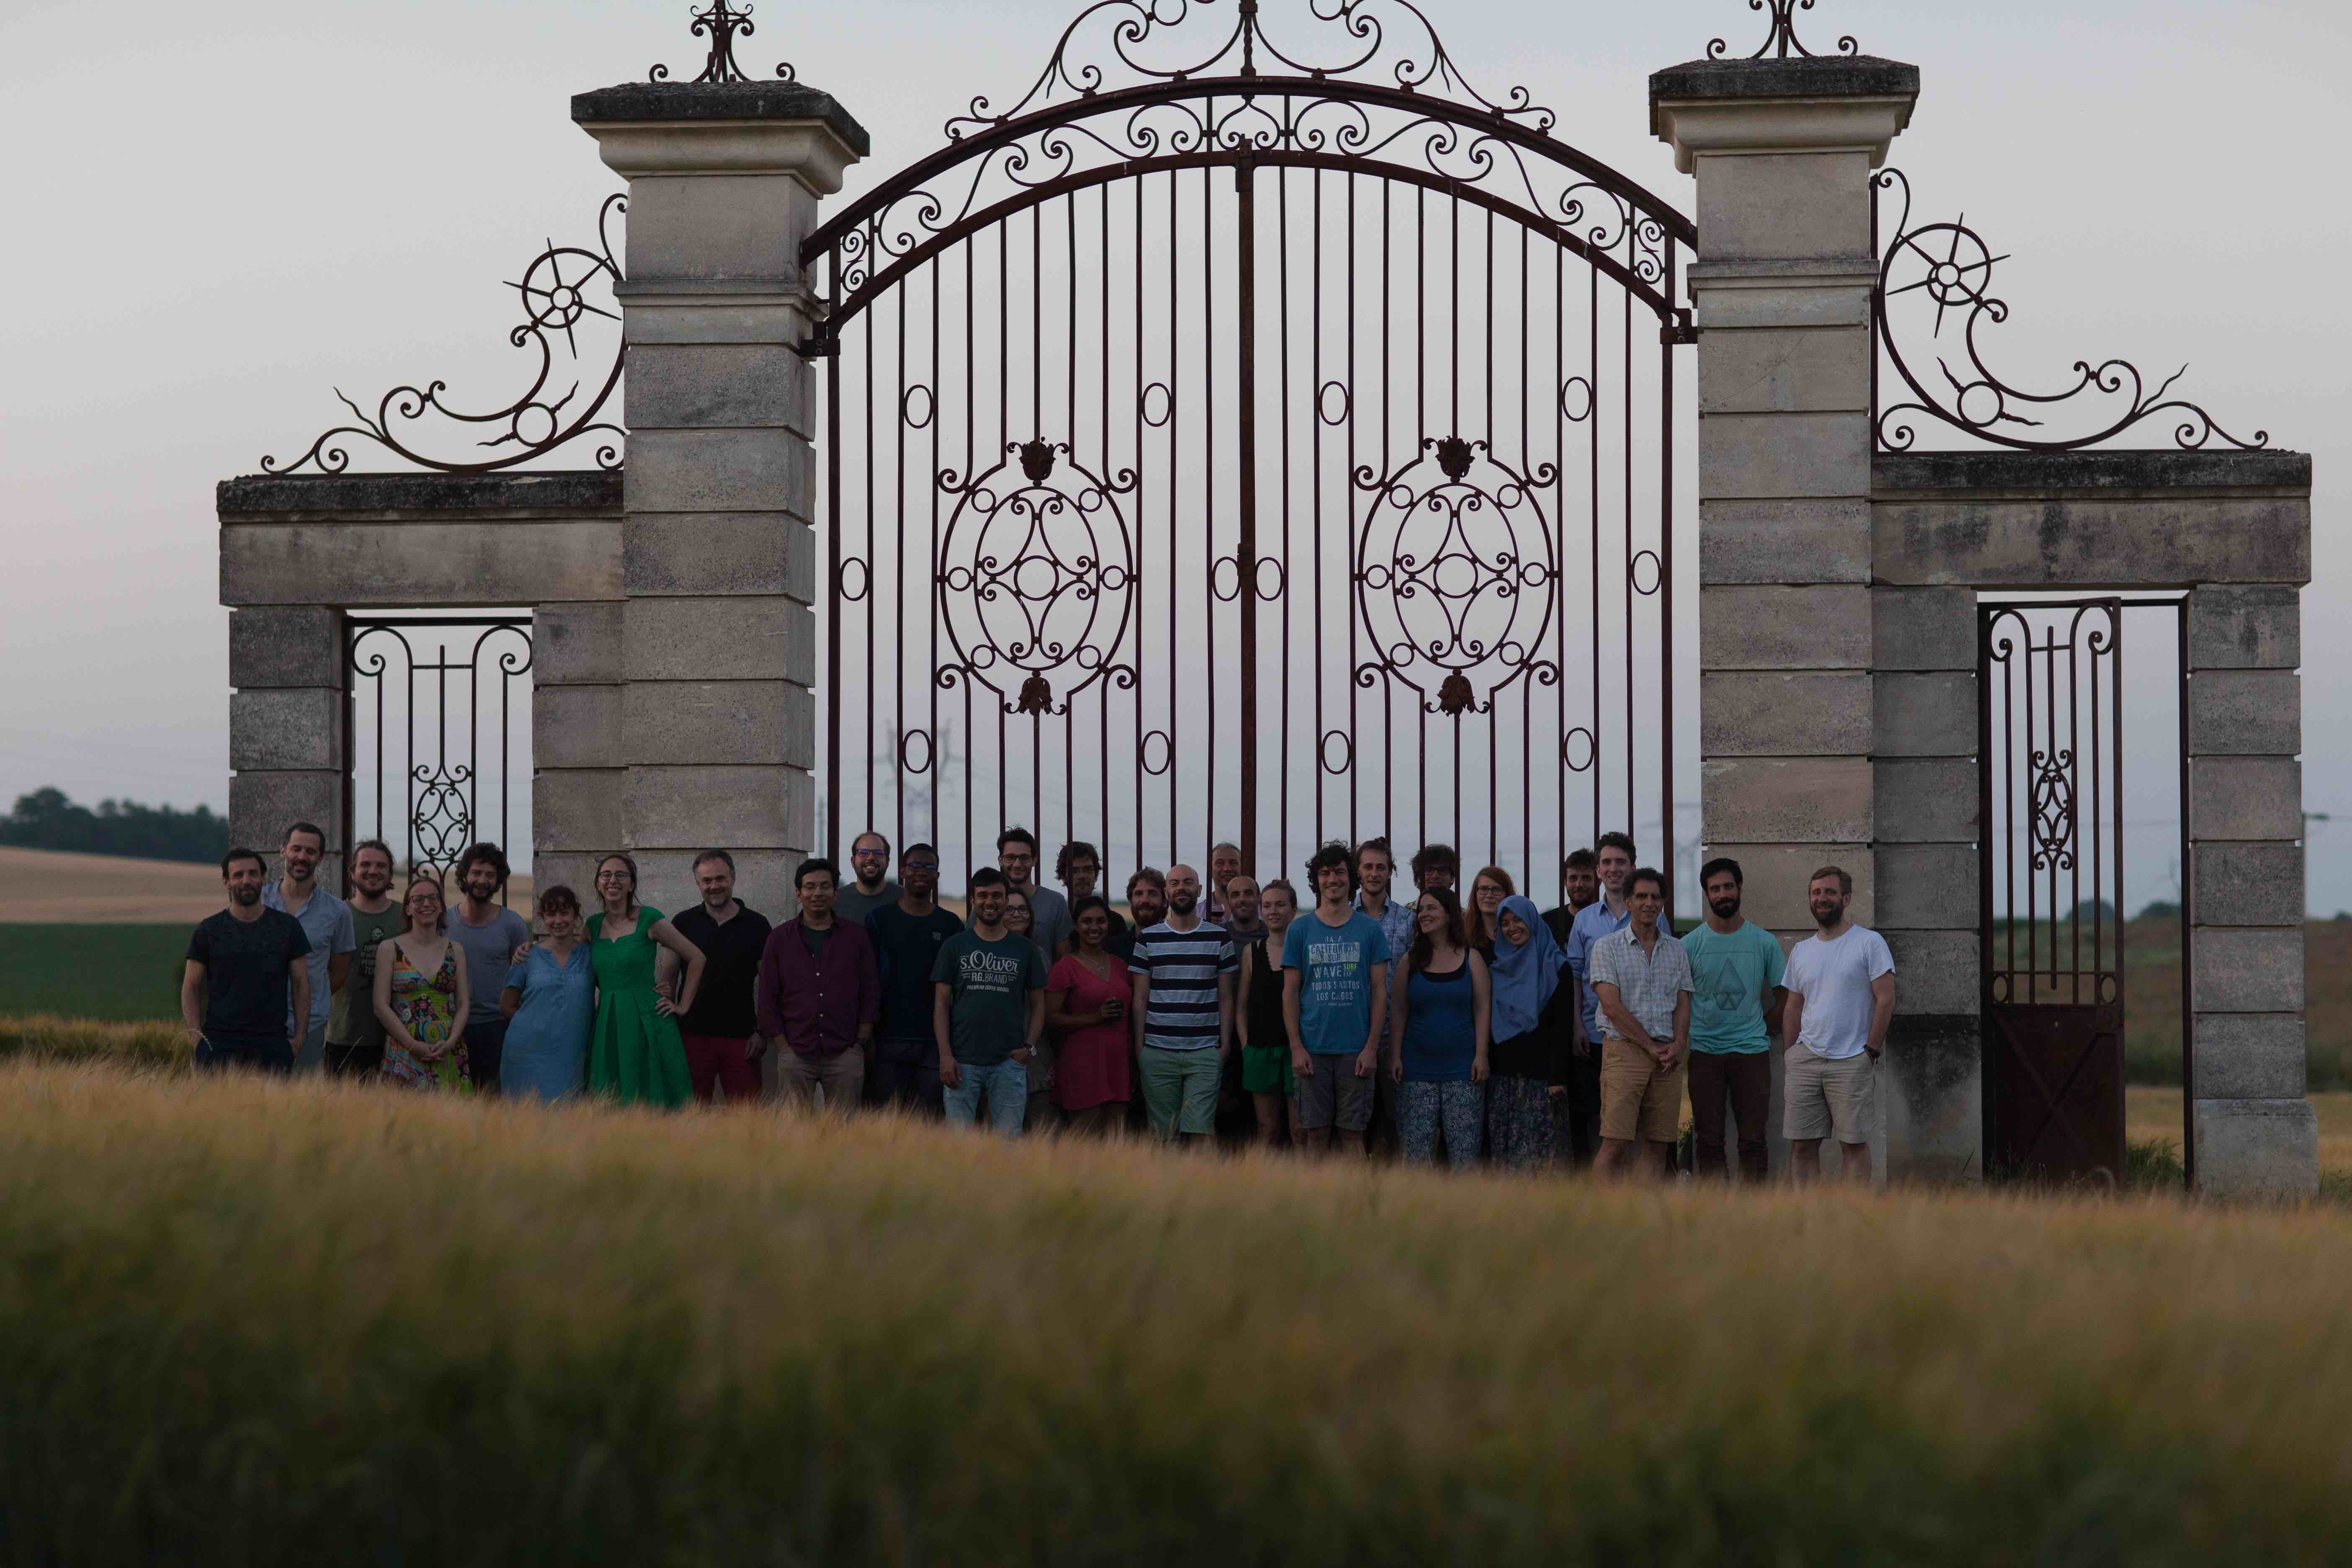
\includegraphics[width=0.9\textwidth]{figures/exmodelo-group_IMG_4067_LR.jpg}



}




%\backupbegin


%%%%%%%%%%%%%%%%%%%%%
\begin{frame}[allowframebreaks]
\frametitle{References}
\bibliographystyle{apalike}
\bibliography{biblio}
\end{frame}
%%%%%%%%%%%%%%%%%%%%%%%%%%%%


%\backupend





\end{document}


